\documentclass[11pt, a4paper]{report}

\usepackage{graphicx}
\graphicspath{ {images/} }
\usepackage{caption}
\usepackage{subcaption}

\usepackage[utf8]{inputenc}
\usepackage{csquotes}

\usepackage[square,sort,comma,numbers]{natbib}
\bibliographystyle{IEEEtran}

\usepackage{amsmath}
\newcommand\addtag{\refstepcounter{equation}\tag{\theequation}}
\usepackage{txfonts}

\usepackage{multirow}
\usepackage{placeins}

\setlength{\parindent}{0ex}
\setlength{\parskip}{1ex}

%Rechtangle painting
\usepackage{tikz}
\usepackage[framemethod=tikz]{mdframed}

\usepackage{listings}

\usepackage{hyperref}
\usepackage{glossaries}
\makenoidxglossaries

\mdfdefinestyle{mdthight}{
    linewidth=1pt,
    innerleftmargin=0bp,
    innerrightmargin=0bp,
    innertopmargin=0bp,
    innerbottommargin=0bp
}

\mdfdefinestyle{border}{
    linewidth=1pt
}

\loadglsentries{Glossary}

\begin{document}

\title{
    
\includegraphics[width=1.75in]{fhnw_fhnw_logo_en.png} \\
    \vspace*{1in}
    \textbf{Report Street Networks}}
\author{
    Authors: \\
    Samuel Merki\\
    Janis Peyer\\
    \vspace*{0.4in} \\
    Coordinator: \\
    Prof. Dr. Stefan Arisona
    \vspace*{0.4in} \\
    Client: \\
    Chair of Information Architecture,
    ETH Zürich
    \vspace*{0.4in} \\
    Course of Studies: \\ Bachelor of Science in Computer Science
    \vspace*{0.4in} \\
    Institute of 4D Technologies \\
    \textbf{University of Applied Sciences and Arts  }\\
    Northwestern Switzerland FHNW
} \date{Friday 19.08.2016}
\maketitle

\begin{abstract}
    In this document different grammars to describe buildings, streets or plants were discussed, analysed and evaluated for their usefulness.

    In the Computational Planning Tools (CPlan), genetic algorithms to grow new districts and cities exist. Those genetic algorithms need fractions of street networks as chromosomes. To generate these chromosomes different clustering algorithms were implemented and tested. First the centroid-based (K-Means) algorithm was developed. Afterwards hierarchical clustering algorithms (Single-Linkage, WPGMA and UPGMA) were realised and the results were compared. To reduce the memory footprint, specialised data structures were developed.

    An analysing method was then created to select useful areas like the city centre or business areas. It allows to compare different clusters and their measurements. Properties like the block area mean or the density (total area divided by total street length) are among these measurements.
\end{abstract}


\tableofcontents


\chapter{Introduction}
In this thesis the initial task was to learn how street network and buildings can be described as grammar for later analysis and regeneration. There exist many different approaches like Shape Grammar \ref{sec:shape_grammar} (building faces generation), L-Systems \ref{sec:L-Systems} (plants growing), Space Syntax \ref{sec:space_syntax} and many others. 

The \textit{Chair of Information Architecture} provided a street generation and analysing tool named CPlan \ref{CPlan}. To become acquainted with the application and to allow using the existing genetic algorithms a tree generating algorithm was developed by us. 

Selecting interesting areas from different cities and recombining them into a new one would allow a fast creation of new cities. To reach this aim many steps are needed. First of all the cities must be separated into reasonable parts based on vertex position or edge length. The approach of this thesis is to use clustering algorithms from the area of machine learning. Then the different area should be valued to select useful areas.

In this document flat \ref{sec:K-Means} (K-Means) and hierarchical \ref{sec:hierarchicalClustering} (WPGMA, UPGMA) clustering algorithms where compared \ref{sec:measurements-speed} and extended to correct wrong assignments \ref{sec:K-Means_shortest_path} or to reduce the memory footprint \ref{sec:memory_usage}.

The implemented clusters are then measured \ref{sec:measurements} based on the suggestions \ref{sec:clusterRating} provided by the ETH-Zurich and compared \ref{sec:measurements-cluster-analysis}. Additionally the results can now be exported into a JSON-File for further use.

To recombine the separated areas/districts to a new city a student at ETH-Zurich is currently working on a regrow algorithm \ref{sec:future_work}. 

\FloatBarrier
\chapter{Background}
This chapter describes state of the art concepts and algorithms, which were studied and used during this thesis. The background is divided into five sections.

Firstly grammars, which can be used to analyse or generate street networks are discussed. In that section \textit{Shape Grammars}, \textit{L-Systems} and the theory \textit{Space Syntax} are explained and analysed.

Secondly the application \gls{acr:CPlan} is described. This software is a computational analysis and synthesis tool for cities. During this thesis it was extended with multiple algorithms.

Thirdly clustering algorithms are explained. Those unsupervised machine learning algorithms have the purpose to separate data with specific characteristics into meaningful groups. In this section the clustering algorithms K-Means and hierarchical clustering (Single-Linkage, WPGMA, UPGMA) are discussed. In later chapters the usage and implementation of those algorithms will be explained.

Fourthly street networks measurement methods, that allow to analyse and compare street subgraphs are described.

Lastly the idea of all pairs shortest path algorithms are explained and compared against a single-source shortest path algorithm.

\section{Shape Grammars} \label{sec:shape_grammar}
The main key of a shape grammars is to generate paintings by a new defined grammar based on shapes, selection rules, painting rules and limiting shapes. A shape grammar is a language based on an alphabet of shapes and generated shapes \citep{shapeGrammars:1972}.

A class of paintings defines the pair (S,M). S represents the shape specifications and M the material specifications. The shape specification contains a shape grammar, defining a language of two dimensional shapes, and a selection rule. M specifies a finite list of material specifications and one limiting shape on a canvas.

\subsection{Shape Grammar Definition}
\label{sec:Shape_Grammar_Definition}
A Shape Grammar is defined over an alphabet of shapes and generated n-dimensional shapes according to \citep{shapeGrammars:1972}.
\begin{quote} 
    Definition. A shape grammar (SG) is a 4-tuple: $SG = (V_T, V_M, R, I)$ where
    \begin{enumerate}
        \item $V_T$ is a finite set of shapes.
        \item $V_M$ is a finite set of shapes such that $V_T $* $\cap$  $V_M = \emptyset$
        \item R is a finite set of ordered pairs (u,v) such that
        
        u is a shape consisting of an element of $V_T $* combined with an element of $V_M$ and
        
        v is a shape consisting of (A) the element of $V_T $* contained in u or (B) the element of $V_T $* contained in u combined with an element of $V_M$ or (C) the element of $V_T $* contained in u with an additional element of $V_T$* and an element of $V_M$.
        
        \item I is a shape consisting of elements of $V_T $* and $V_M$.
    \end{enumerate}
\end{quote}

\subsection{Selection Rules}
\label{sec:Shape_Grammar_Selection_Rules}
A painting is generated based on an undefined count of shape rules. This requires a mechanism to select a correct shape. The depth is defined by levels which are being assigned during generation based on their rules according to \citep{shapeGrammars:1972}:
\begin{displayquote}
    \begin{enumerate}
        \item The terminals in the initial shape are assigned to level 0.
        \item If a shape rule is applied, and the highest level assigned to any part ot the terminal corresponding to the level side of the rule is N, then
        \begin{enumerate}
            \item If the rule is of type A, any part of the terminal enclosed by the marker in the left side of the rule is assigned to N.
            \item If the rule is of type B, any part of the terminal enclosed by the marker in the left side of the rule is assigned to N and any part of the terminal enclosed by the marker is assigned to N+1.
            \item If the rule is of type C, the terminal added is assigned to N+1.
        \end{enumerate}
        \item No other level assignments are made.
    \end{enumerate}
\end{displayquote}

\subsection{Painting Rules}
\label{sec:Shape_Grammar_Painting_Rules}
Painting rules describe witch shape should be painted inside of a defined area. Like in a Venn diagram the rules contain multiple levels 0 - n. By combining these levels the painting colour is described\citep{shapeGrammars:1972}. The assignments are made by the common operators. An example can be viewed in figure \ref{fig:shape_grammar_gen_specifications}

\subsection{Limiting Shapes}
\label{sec:Shape_Grammar_Limiting_Shapes}
These shapes define a limiting area on the canvas, where shape painting is allowed. 
The area could have any form, but normally it is defined as a rectangle. Like a camera view the limiting shape defines the scale of a painting and its viewpoint. Therefore the initial/start shape could be outside of the limiting shape.

\subsection{Example}
These specifications \ref{fig:shape_grammar_gen_specifications} have been used to generate the output image \ref{fig:Shape Grammars/Example}. In the output image \ref{fig:Shape Grammars/Example} the relevant steps can be observed. The levels are generated as described in the section \ref{sec:Shape_Grammar_Selection_Rules}. Level 0 is represented by steps 0 and 1. Steps 2 to 5 are on level 1 and finally steps 18 and 19 are on Level 2.
\begin{figure}[!ht]
    \centering
    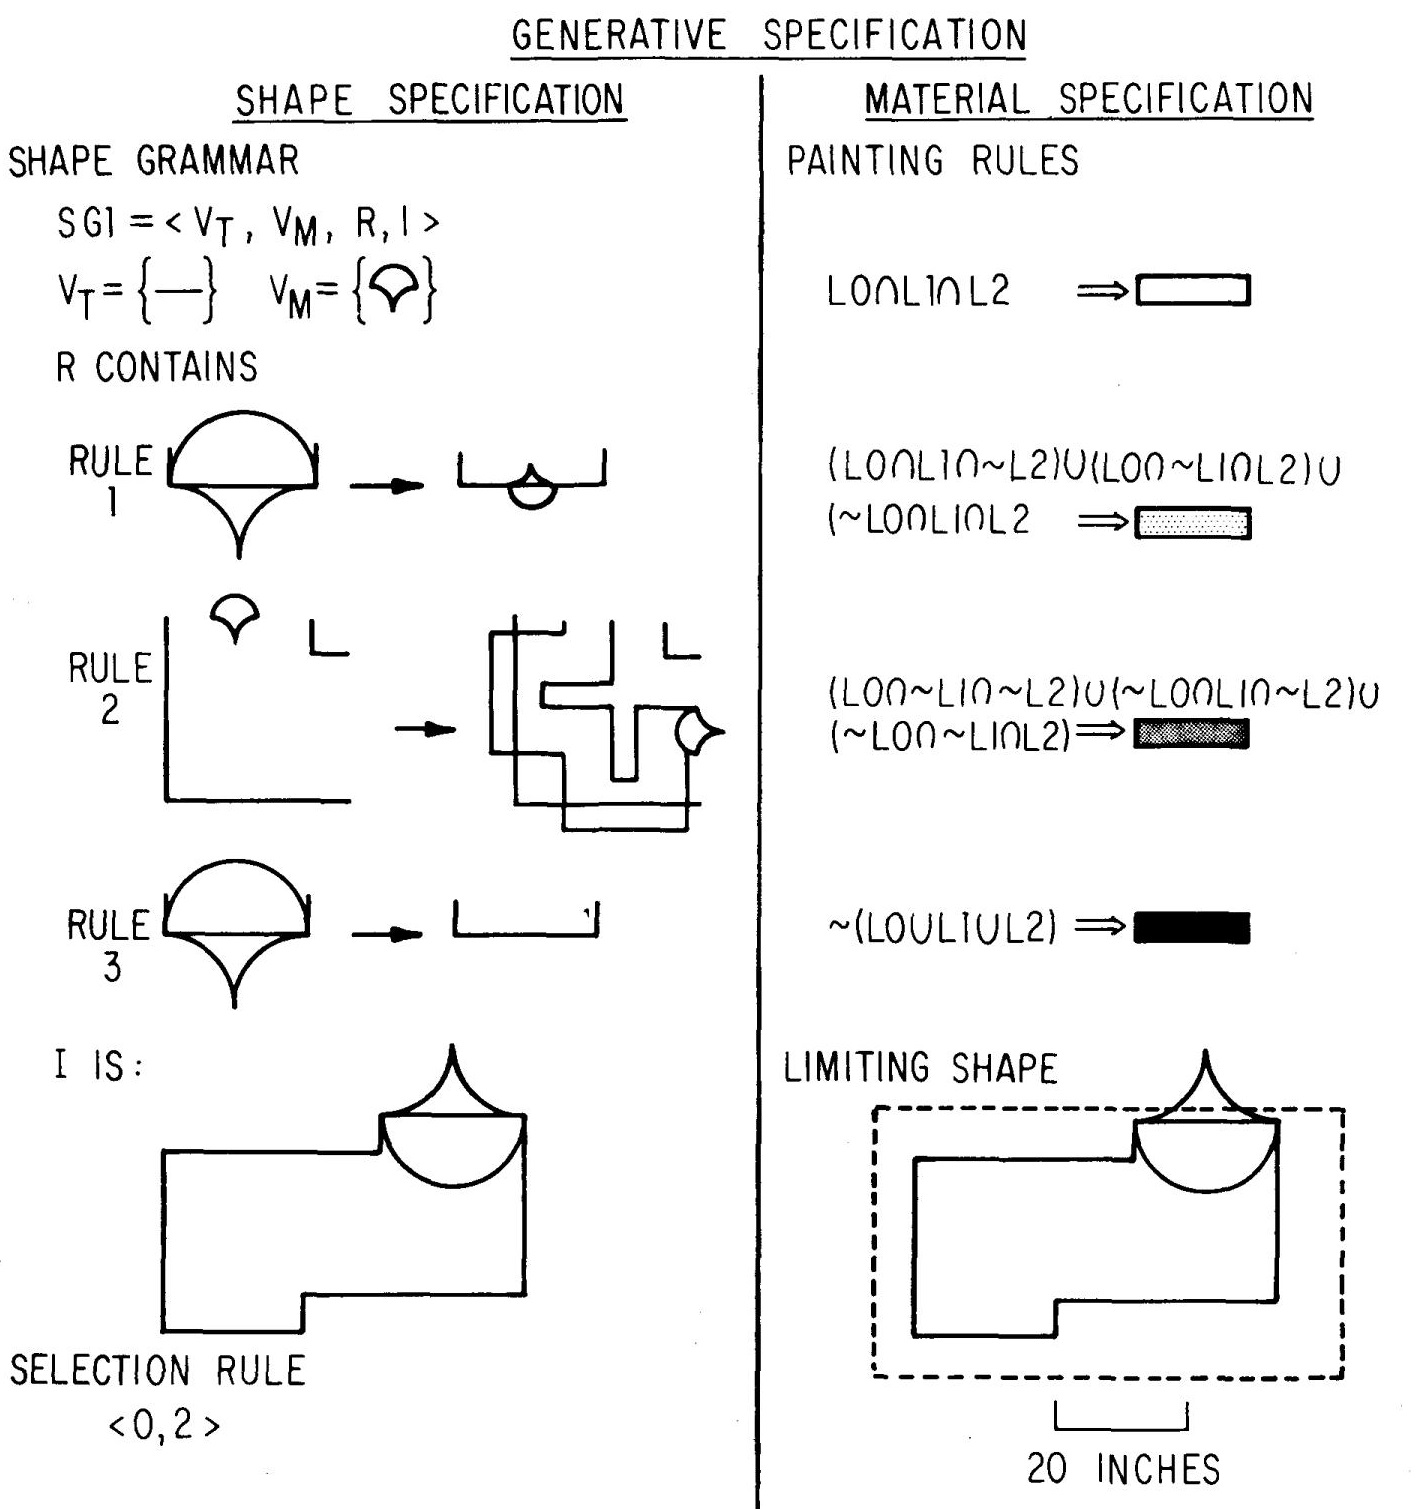
\includegraphics{shape_grammar_generativ_spec.jpg}
    \caption{Generative Specifications - \textit{Source: Shape Grammar} \citep{shapeGrammars:1972}}
    \label{fig:shape_grammar_gen_specifications}
\end{figure}

\begin{figure}[!ht]
    \centering
    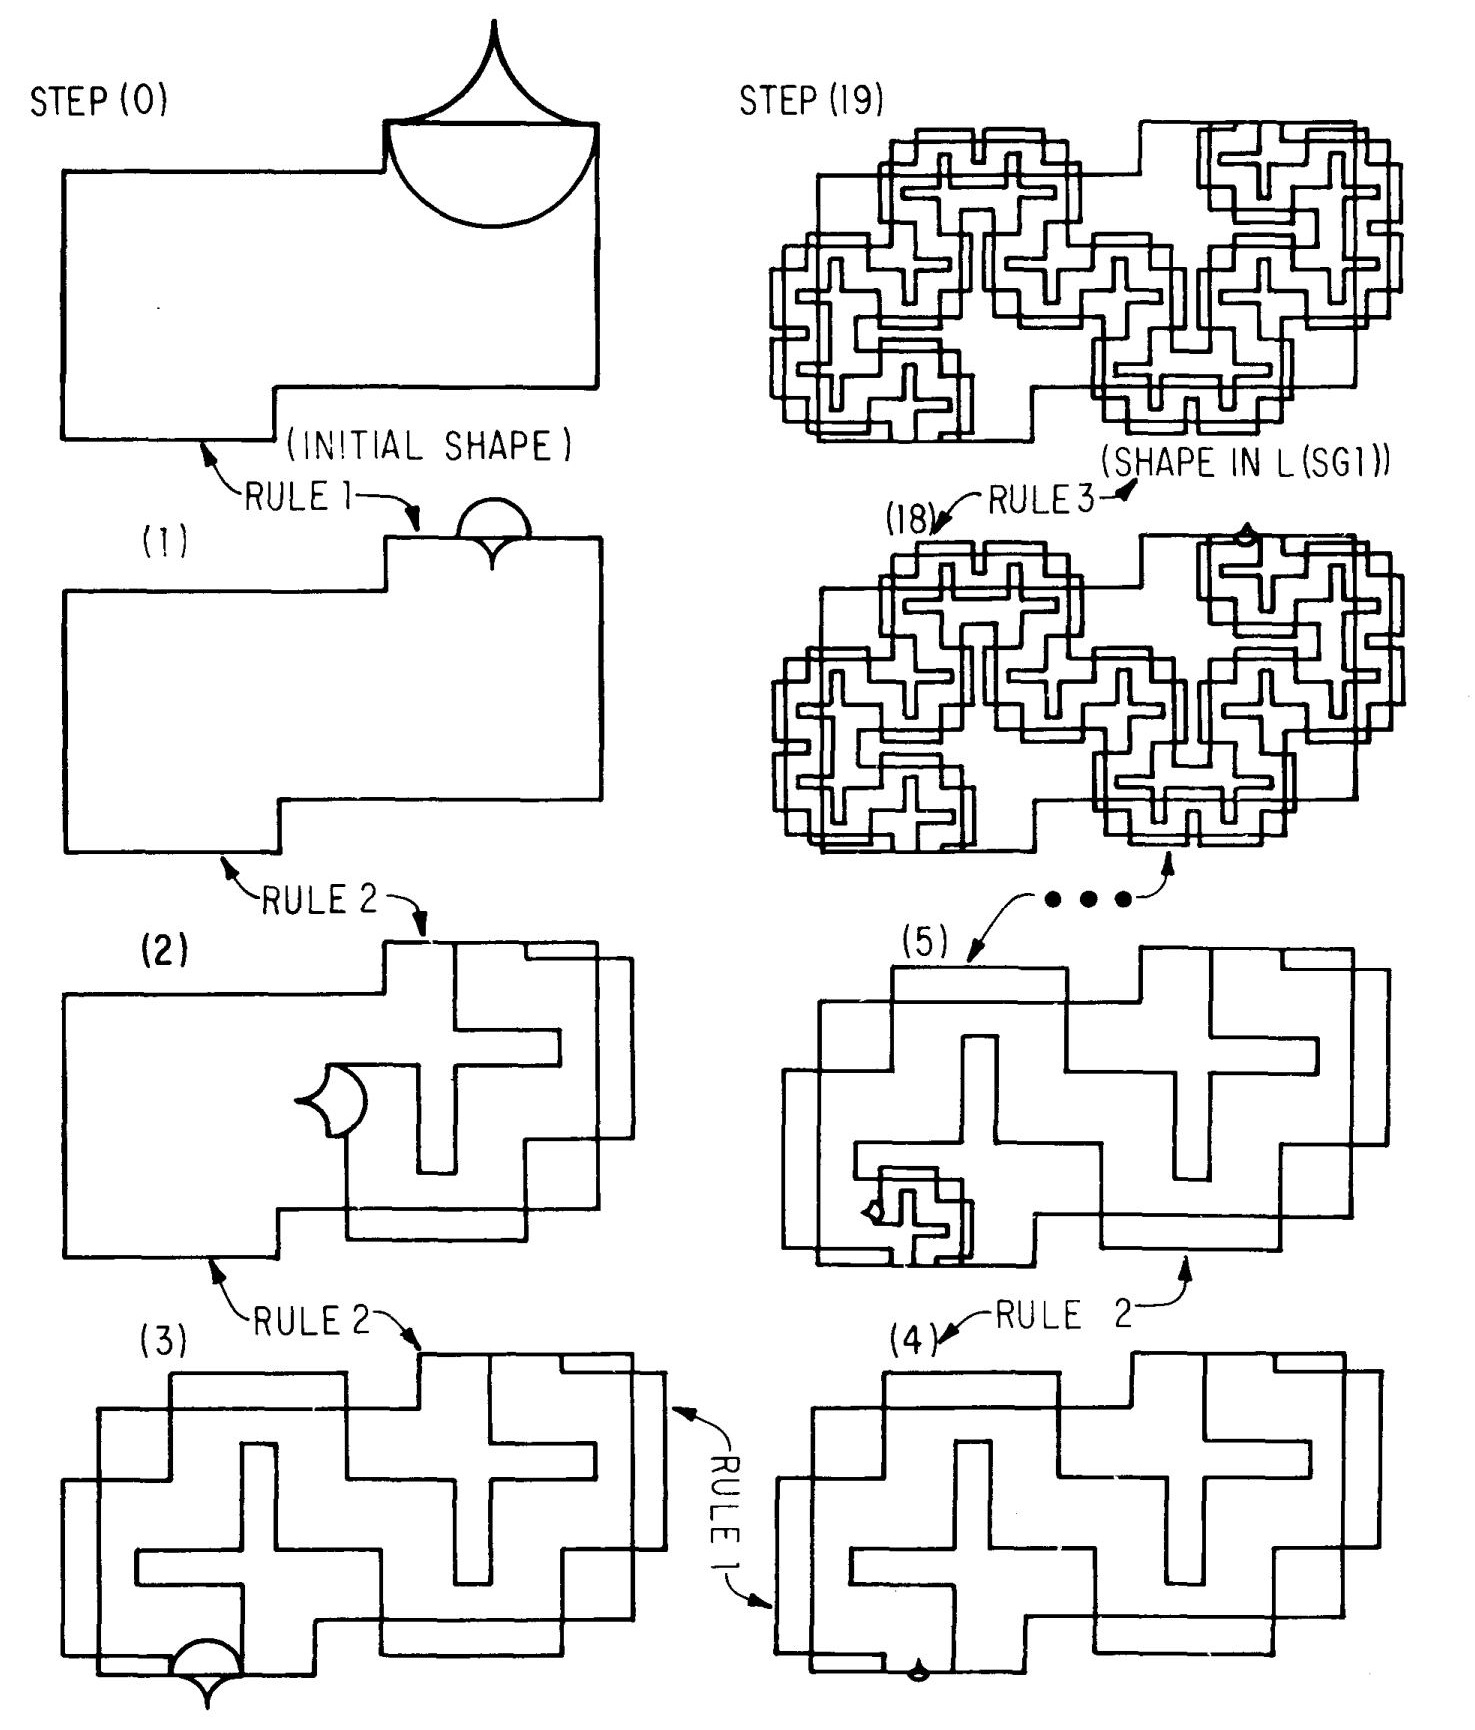
\includegraphics[width=\textwidth]{sg_example.jpg}
    \caption{ Generated Painting - \textit{Source: Shape Grammar} \citep{shapeGrammars:1972}}
    \label{fig:Shape Grammars/Example}
\end{figure}

\FloatBarrier
\pagebreak
\subsection{Street Generation}
In the following section we debate the usefulness of generating street networks by shape grammars.
\subsubsection{Features}
\begin{itemize}
    \item Can describe and generate veneer in high details.
    \item With R-Shapes windows and high detail 3D-Models can be generated easily.
\end{itemize}

\subsubsection{Problems}
\begin{itemize}
    \item The given methods generate monotonous streets in most cases. 
    \item A huge number of R-Shapes is required to generate a useful street network.
    \item Areas with different characteristics (historic district, rectangular raster like New York or radial to center like Paris) are difficult to generate.
    \item The R-Rules for the transitions between area characteristics should not repeat themselves and are for that reason difficult to build.
\end{itemize}

\pagebreak
\section{L-Systems} \label{sec:L-Systems}
L-System is a well established modelling approach for the synthesis of realistic plant images. There are many papers describing L-Systems and how they are applied to generate plant life: "In these cases L-System productions capture the \textit{development} of plant components over time." \citep{PrusinkiewiczEtAl:2001} Productions are applied in parallel, so that all plant parts grow and age equally. The growth is stopped at a defined terminal age. This age is the number of iterations, where in each iteration productions are applied.

The context-free productions in \citep{PrusinkiewiczEtAl:2001} are defined using the following syntax.
\begin{equation} \label{eq:lsystem context free}
pred : \{block1\}\ cond\ \{block2\} \leadsto succ
\end{equation}
The symbol \textit{pred} (predecessor) defines the module that will get replaced by the modules defined in \textit{succ} (successor). This replacement is only applied, if the (optional) condition is met. \textit{block1} and \textit{block2} are C statement blocks, of which the first block is executed before and the second after the condition is evaluated. \citep{PrusinkiewiczEtAl:2001} gives the following example.
\begin{equation} \label{eq:lsystem example 1}
A(x) : \{y = x + 2;\}\ y \geq 5\ \{z = y / 3;\}\ \leadsto B(z)C(z + 1)
\end{equation}
If this example production was applied to the module $A(4)$, it would result in the modules $B(2)C(3)$.

The modelling language, described in \citep{PrusinkiewiczEtAl:2001}, also supports context-sensitive productions. The following listing defines the syntax of such a production.
\begin{equation} \label{eq:lsystem context sensitive}
lcont < pred > rcont : \{block1\}\ cond\ \{block2\} \leadsto succ
\end{equation}
\textit{lcont} (left context) and \textit{rcont} (right context) each define a list of modules that have to precede or respectively follow the \textit{pred} (module being replaced). Context modules are limited to query symbols, which are explained later on. \citep{PrusinkiewiczEtAl:2001} gives the following example.
\begin{equation} \label{eq:lsystem example 2}
A(x) < B(y) > C(z) : x + z > 0 \leadsto M(y / 2)N(y / 2)
\end{equation}
If the example of listing \ref{eq:lsystem example 2} was applied to the module composition $A(2)B(4)C(0)$, it would result in the modules $A(2)M(2)N(2)C(0)$.

A way to generate images with L-Systems is to use a LOGO-style turtle as a graphical model. Certain modules of the L-System are interpreted as commands to this turtle.

\pagebreak
\section{Space Syntax} \label{sec:space_syntax}
The axial line-based space syntax was first introduced in 1976 by B. Hiller, A. Leaman, P. Stansall and M. Bedford in the paper \textit{Space syntax} \citep{spaceSyntax:1976}. This theory is based on a morphic language and describes methods to analyse and generate urban areas and buildings.

The theory was later extended and integrated into \textit{Geographic Information System} (GIS) as point-based space syntax (graph). This systems are used to plan and analyse the human interaction with the environment.

\subsection{Axial line-based space syntax and limitations}
In space syntax streets are represented by axial lines. 
\textit{"Axial lines are used to represent directions of uninterrupted movement and visibility, so they represent the longest visibility lines in two-dimensional urban spaces."} \citep{integrationSpaceSyntaxGIS:2002}
This approach has allowed many analysis methods of urban systems like way-finding process or criminal analysis. An axial map represents a fully filled free space with many axial lines \ref{fig:barnsbury_axial_map}. For a more detailed analysis the lines can by broken into segments at the intersections \ref{fig:barnsbury_segmented_axial_map}. To generate the axial map always the longest not visited space is selected and line drawn till the hole space is covered.

Axial maps have many limitations. First the complexity to create an axial map is high because of the generating procedure. If an additional area is added the hole process of detection should be repeated because a longer start line could exist. The process is non-deterministic because a curve could be separated into a unknown count of lines.

\begin{figure}[ht]
    \centering
    \begin{subfigure}[b]{0.4\textwidth}
        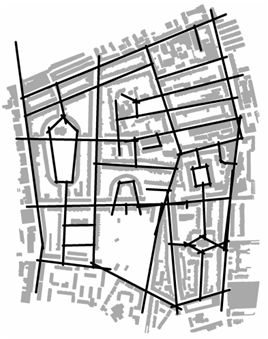
\includegraphics[width=\textwidth]{The-figure-ground-plan-of-Barnsbury-Axial-map.jpg}
        \caption{Barnsbury axial map}
        \label{fig:barnsbury_axial_map}
    \end{subfigure}
    \quad
    \begin{subfigure}[b]{0.4\textwidth}
        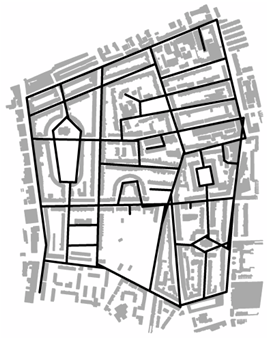
\includegraphics[width=\textwidth]{The-figure-ground-plan-of-Barnsbury-Axial-segment-map.jpg}
        \caption{Barnsbury segmented axial map}
        \label{fig:barnsbury_segmented_axial_map}
    \end{subfigure}
    \caption{Space Syntax: Axial Map - \textit{Source: UCL Space Syntax \citep{SpaceSyntaxExampels}}}
    \label{fig:SpaceSyntaxAxialMap}
\end{figure}

\subsection{Point-based space syntax}
A point-based space syntax is a decision based approach as described by Bin Jiang and Christope Claramunt in \textit{Integration of Space Syntax into GIS: New Perspectives for Urban Morphology} \citep{integrationSpaceSyntaxGIS:2002}. Every time a point in a street network is visited the visitor can decide which direction he will travel next. The distances between two point can directly be measured and described. Every point can be assigned to an ID and marked with x and y coordinates \ref{fig:space_syntax_gis_characteristic_points}. This approach is at least equivalent to the predefined syntax created by B. Hiller et al.\citep{spaceSyntax:1976} because a visibility graph can be create to represent axial lines \ref{fig:space_syntax_gis_visibility_graph}. The point-based space syntax therefore is a graph based approach.

\begin{figure}[ht]
    \centering
    \begin{subfigure}[b]{0.4\textwidth}
        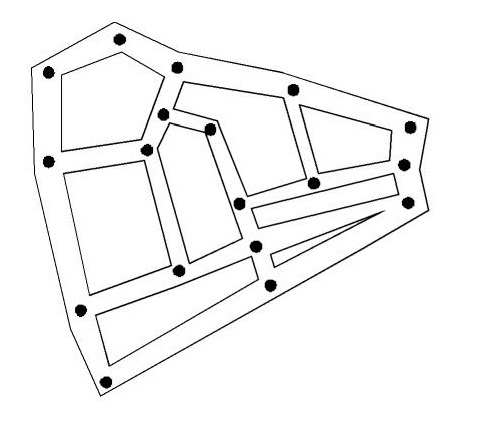
\includegraphics[width=\textwidth]{space_syntax_gis_characteristic_points.jpg}
        \caption{Characteristic points}
        \label{fig:space_syntax_gis_characteristic_points}
    \end{subfigure}
    \quad
    \begin{subfigure}[b]{0.4\textwidth}
        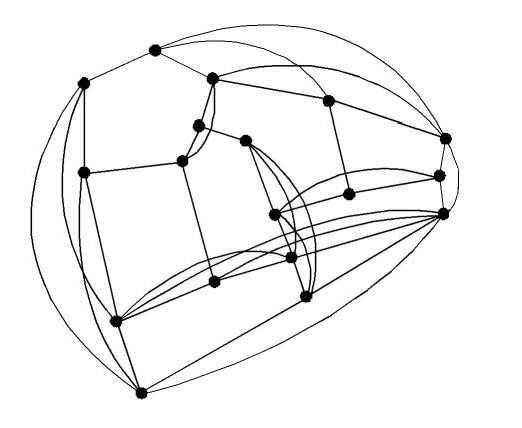
\includegraphics[width=\textwidth]{space_syntax_gis_visibility_graph.jpg}
        \caption{Visibility graph}
        \label{fig:space_syntax_gis_visibility_graph}
    \end{subfigure}
    \caption{Point-based space syntax - \textit{Source: Integration of Space Syntax into GIS \citep{integrationSpaceSyntaxGIS:2002}}}
    \label{fig:space_syntax_gis}
\end{figure}

\subsection{Comparison with CPlan}
The application CPlan \ref{CPlan} does handle the street networks as graphs. As a result the same measurements methods can be applied as mentioned for the point-based space syntax. The clustering algorithms later discussed \ref{sec:K-Means}, \ref{sec:hierarchicalClustering} are applied on vertex/points and unidirectional edges between the points.

\pagebreak
\FloatBarrier
\section{CPlan}
\label{CPlan}
CPlan is a tool written by the Department of Architecture of the ETH-Zurich. The goal of this application is to generate/grow street networks dynamically and extend these networks with buildings.

\pagebreak
\FloatBarrier
\section{K-Means Clustering}
\label{sec:K-Means}
The K-Means clustering algorithm detects clusters / partitions by measuring the euclidean distance between the cluster centroids and the features derived from the input data \cite{k-means++:2007}. The algorithm uses the following approach:

\begin{enumerate}
    \item $k$ data features are used as initial centroids ($k$ is the number of created clusters)
    \item Each data entry is assigned to its nearest centroid
    \item The centroids are moved to the mean (center) of the features of all assigned data entries
    \item Until the maximum number of iterations is reached this process is repeated starting with item 2
\end{enumerate}

\subsection{Local minima problem}
Because the K-Means algorithm can find local minima, this process needs to be executed more than once. The result with the best found solution will be selected.

\subsection{K-Means++} \label{sec:k-means++}
The K-Means algorithm was later extended to set reasonable start centroids. This extensions allows to run a K-Means run with $O(log\ k)$ \cite{k-means++:2007}.

\subsection{KD-Tree} \label{sec:k-means_KD-tree}
A K-Dimensional tree could improve the time complexity of the k-means algorithm \citep{kmeans:2002}. This tree separates k-dimensional data into a structure, where queries for single data points or ranges can be evaluated with way better performance.

\pagebreak
\FloatBarrier
\section{Hierarchical Clustering} \label{sec:hierarchicalClustering}

Hierarchical clustering also known as connectivity based clustering is an area of algorithms, which clusters nodes together that are near to each other. The advantage over K-Means is that graph distances can be used instead of the euclidean distance.

The result of a hierarchical clustering algorithm is a tree also called hierarchy, hence the name. This result can be used to create $1$ to $n$ clusters, where $n$ is the number of data entries. Those data entries are in some cases also called nodes in this document.

\subsection{Strategy}
As described in \cite{clustering:2005}, there are generally two main strategies for hierarchical clustering:

\begin{itemize}
    \item \textbf{Agglomerative}: Bottom up strategy. In the beginning each node is an own cluster. Clusters are combined until only a single cluster remains.
    \item \textbf{Divisive}: Top down strategy. All nodes are contained in one cluster at the start. This cluster is then divided into sub-clusters.
\end{itemize}

The time complexity of the divisive strategy with $O(2^n)$ is not performing well enough for the size of the street networks on which the algorithms have to run. The agglomerative strategy runs in $O(n^2 log(n))$ and in some special cases in $O(n^2)$ time complexity. The hierarchical clustering algorithms implemented for this thesis run in $O(n^2)$ time complexity. They are based on the paper "Optimal implementations of UPGMA and other common clustering algorithms" \cite{clustering:2007}.

\subsection{Reduction Formula}
The reduction formula is used to determine the distance between two clusters.
The following reduction formulae were implemented for this thesis:

\begin{itemize}
    \item \textbf{Single Linkage}
    \begin{multline}
    D_{Single-Linkage}(C_1, (C_2 \cup C_3)) \leftarrow \\
    min \{ D_{Single-Linkage}(C_1, C_2), D_{Single-Linkage}(C_1, C_3) \}
    \end{multline}
    \item \textbf{\acrshort{UPGMA}} (\acrlong{UPGMA})
    \begin{equation}
    \begin{split}
    D_{UPGMA}(C_1, (C_2 \cup C_3)) \leftarrow &\frac{|C_2|}{|C_2|+|C_3|}D_{UPGMA}(C_1, C_2)\ + \\ &\frac{|C_3|}{|C_2|+|C_3|}D_{UPGMA}(C_1, C_3)
    \end{split}
    \end{equation}
    \item \textbf{\acrshort{WPGMA}} (\acrlong{WPGMA})
    \begin{equation}
    D_{WPGMA}(C_1, (C_2 \cup C_3)) \leftarrow \frac{1}{2} (D_{WPGMA}(C_1, C_2) + D_{WPGMA}(C_1, C_3))
    \end{equation}
\end{itemize}

$C_1$, $C_2$ and $C_3$ are clusters, each being a set of nodes. The distance function $d(i, j)$ determines the distance between nodes $i$ and $j$.

For every of these reduction formulae the following holds:

\begin{equation}
\begin{split}
&\textrm{Let }C_1, C_2\textrm{ be clusters}, i \in C_1,\ j \in C_2, \\
&\textrm{if }|C_1| = |C_2| = 1, \\
&\textrm{then }D(C_1, C_2) = d(i, j)
\end{split}
\end{equation}

For both the single linkage and the \acrshort{UPGMA} reduction formula exists a dissimilarity function (listings \ref{eq:df_single_linkage} and \ref{eq:df_upgma}). These are alternative formulations of the reduction formulae which determine the cluster distance by traversing all nodes of both clusters. The created cluster hierarchy is not used in these functions. For the \acrshort{WPGMA} reduction formula no dissimilarity function exists, as shown in \cite{clustering:2007}.

\begin{align}
\label{eq:df_single_linkage}
D_{Single-Linkage}(C_1, C_2) &= \min_{i\in{C1}, j\in{C2}}\{d(i, j)\} \\
\label{eq:df_upgma}
D_{UPGMA}(C_1, C_2) &= \dfrac{1}{|C_1||C_2|} \sum_{i\in{C1}, j\in{C2}}{d(i, j)}
\end{align}

\subsection{Hierarchy}
The output of the hierarchical clustering algorithm is as the name suggests a hierarchy. Figure \ref{fig:hierarchy} shows such an output. For simplicity only five input nodes were used. If this hierarchy was created using an agglomerative strategy the result could have been built as follows:

\begin{enumerate}
    \item Combine the two leftmost nodes
    \item Combine the two rightmost nodes
    \item Combine the cluster formed in step 1 with the middle node
    \item Combine the cluster formed in step 3 with the one combined in step 2
\end{enumerate}

To create a clustering from this output the procedure from above is reversed. In the order, in which the combinations were made, the clusters are split. The hierarchy can be looked at as a single cluster. With each split one hierarchy is divided into two new hierarchies.

Using this method it is possible to create 1 to $n$ clusters from any hierarchy, where $n$ is the number of nodes. Figure \ref{fig:hierarchy_with_clusters} shows an example of this process. From the same hierarchy with five nodes which was used before two clusters were created. A later section (\ref{sec:outout_modification}) shows, that the order in which the hierarchies are split, can be modified.

\begin{figure}[!hb]
    \centering
    \begin{subfigure}[b]{\textwidth}
        \begin{mdframed}[style=border]
            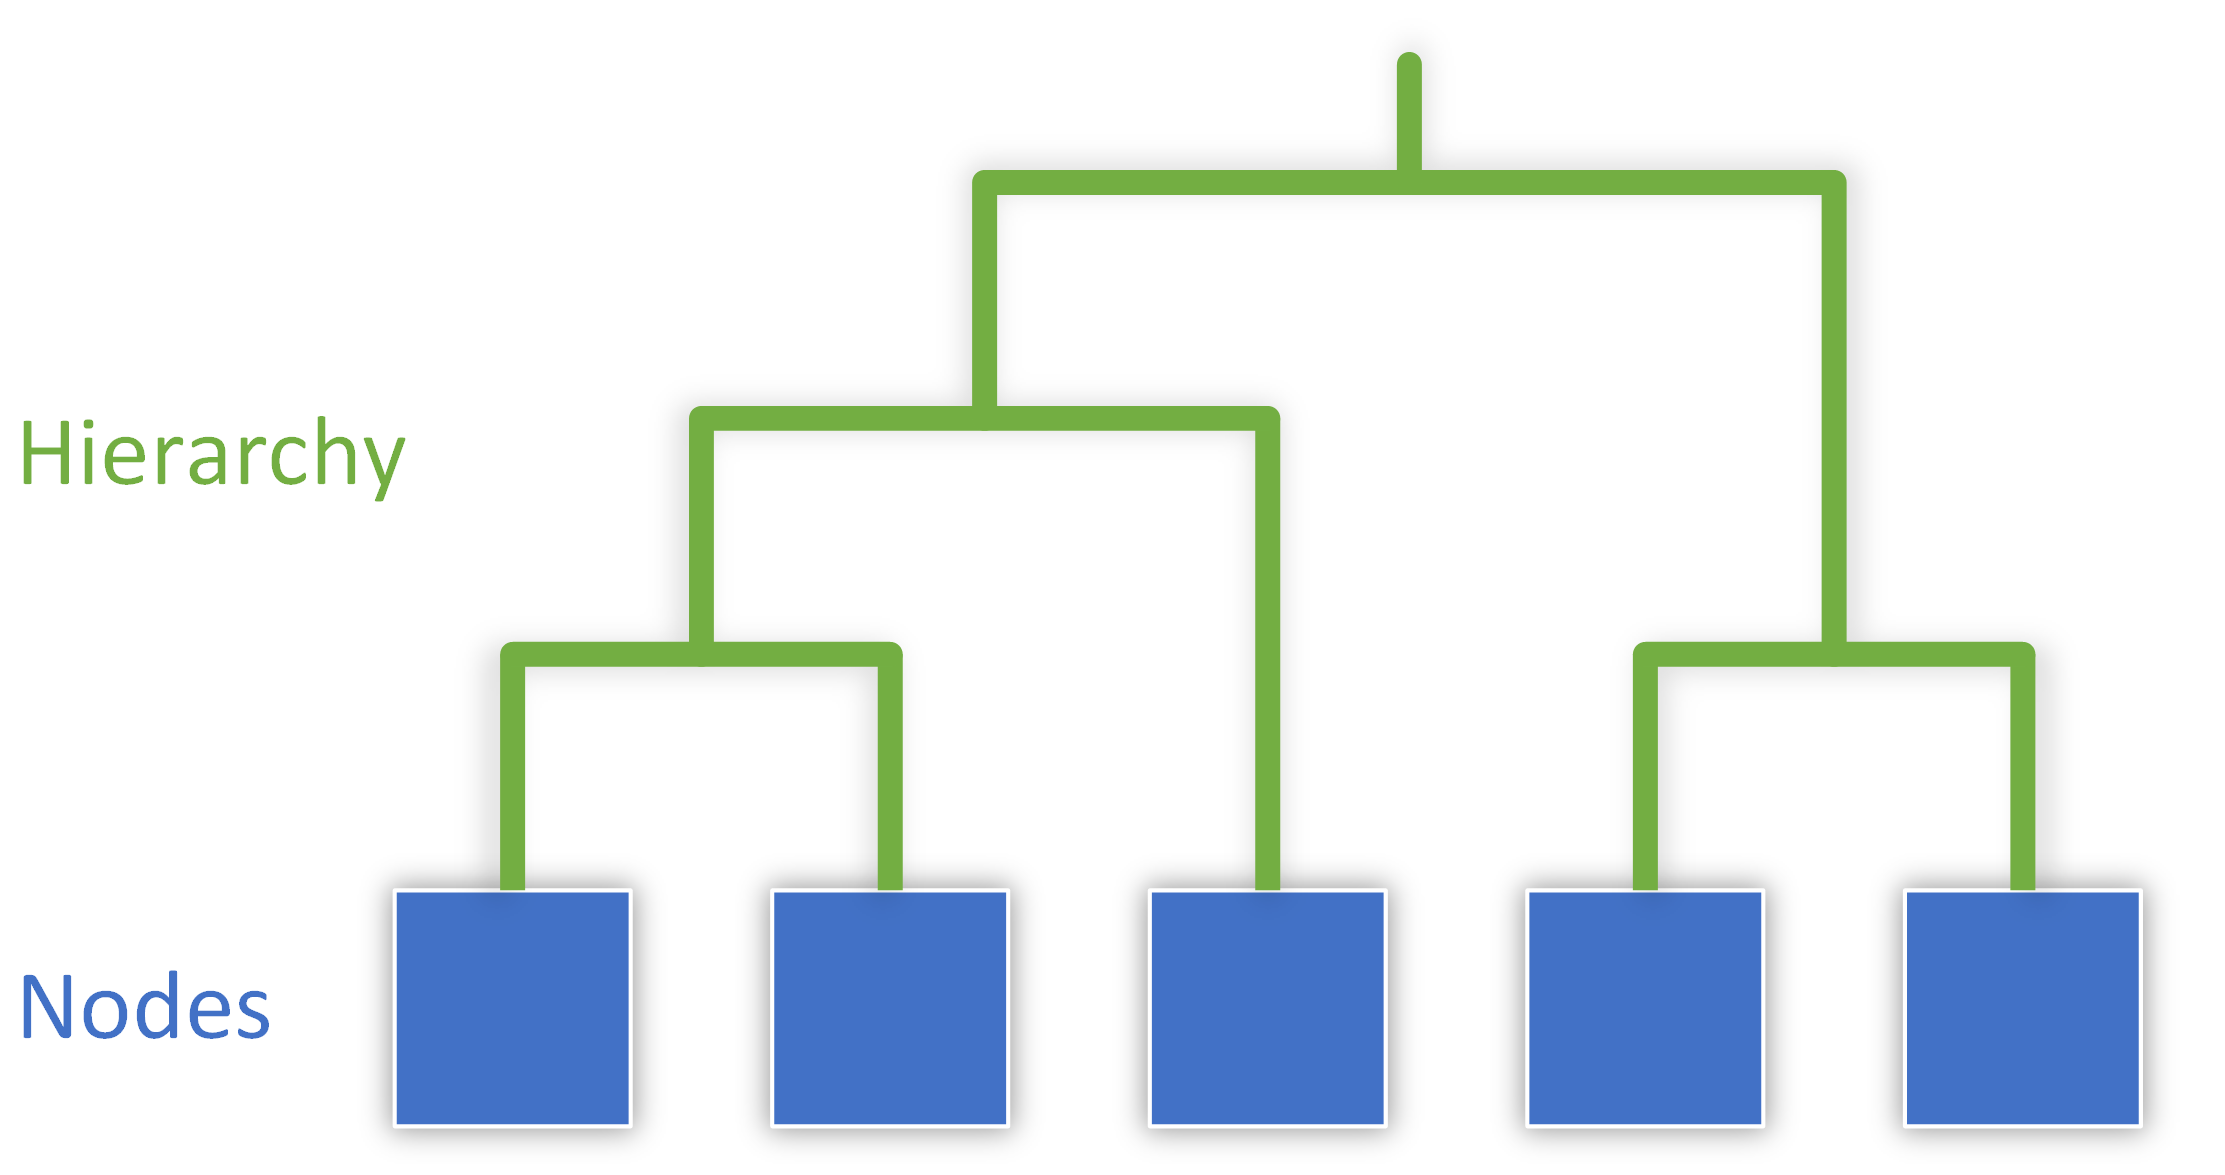
\includegraphics[width=\linewidth]{hierarchy.png}
        \end{mdframed}
        \caption{Hierarchy, which is the output of a hierarchical clustering algorithm}
        \label{fig:hierarchy}
    \end{subfigure}
    \par\medskip
    \begin{subfigure}[b]{\textwidth}
        \begin{mdframed}[style=border]
            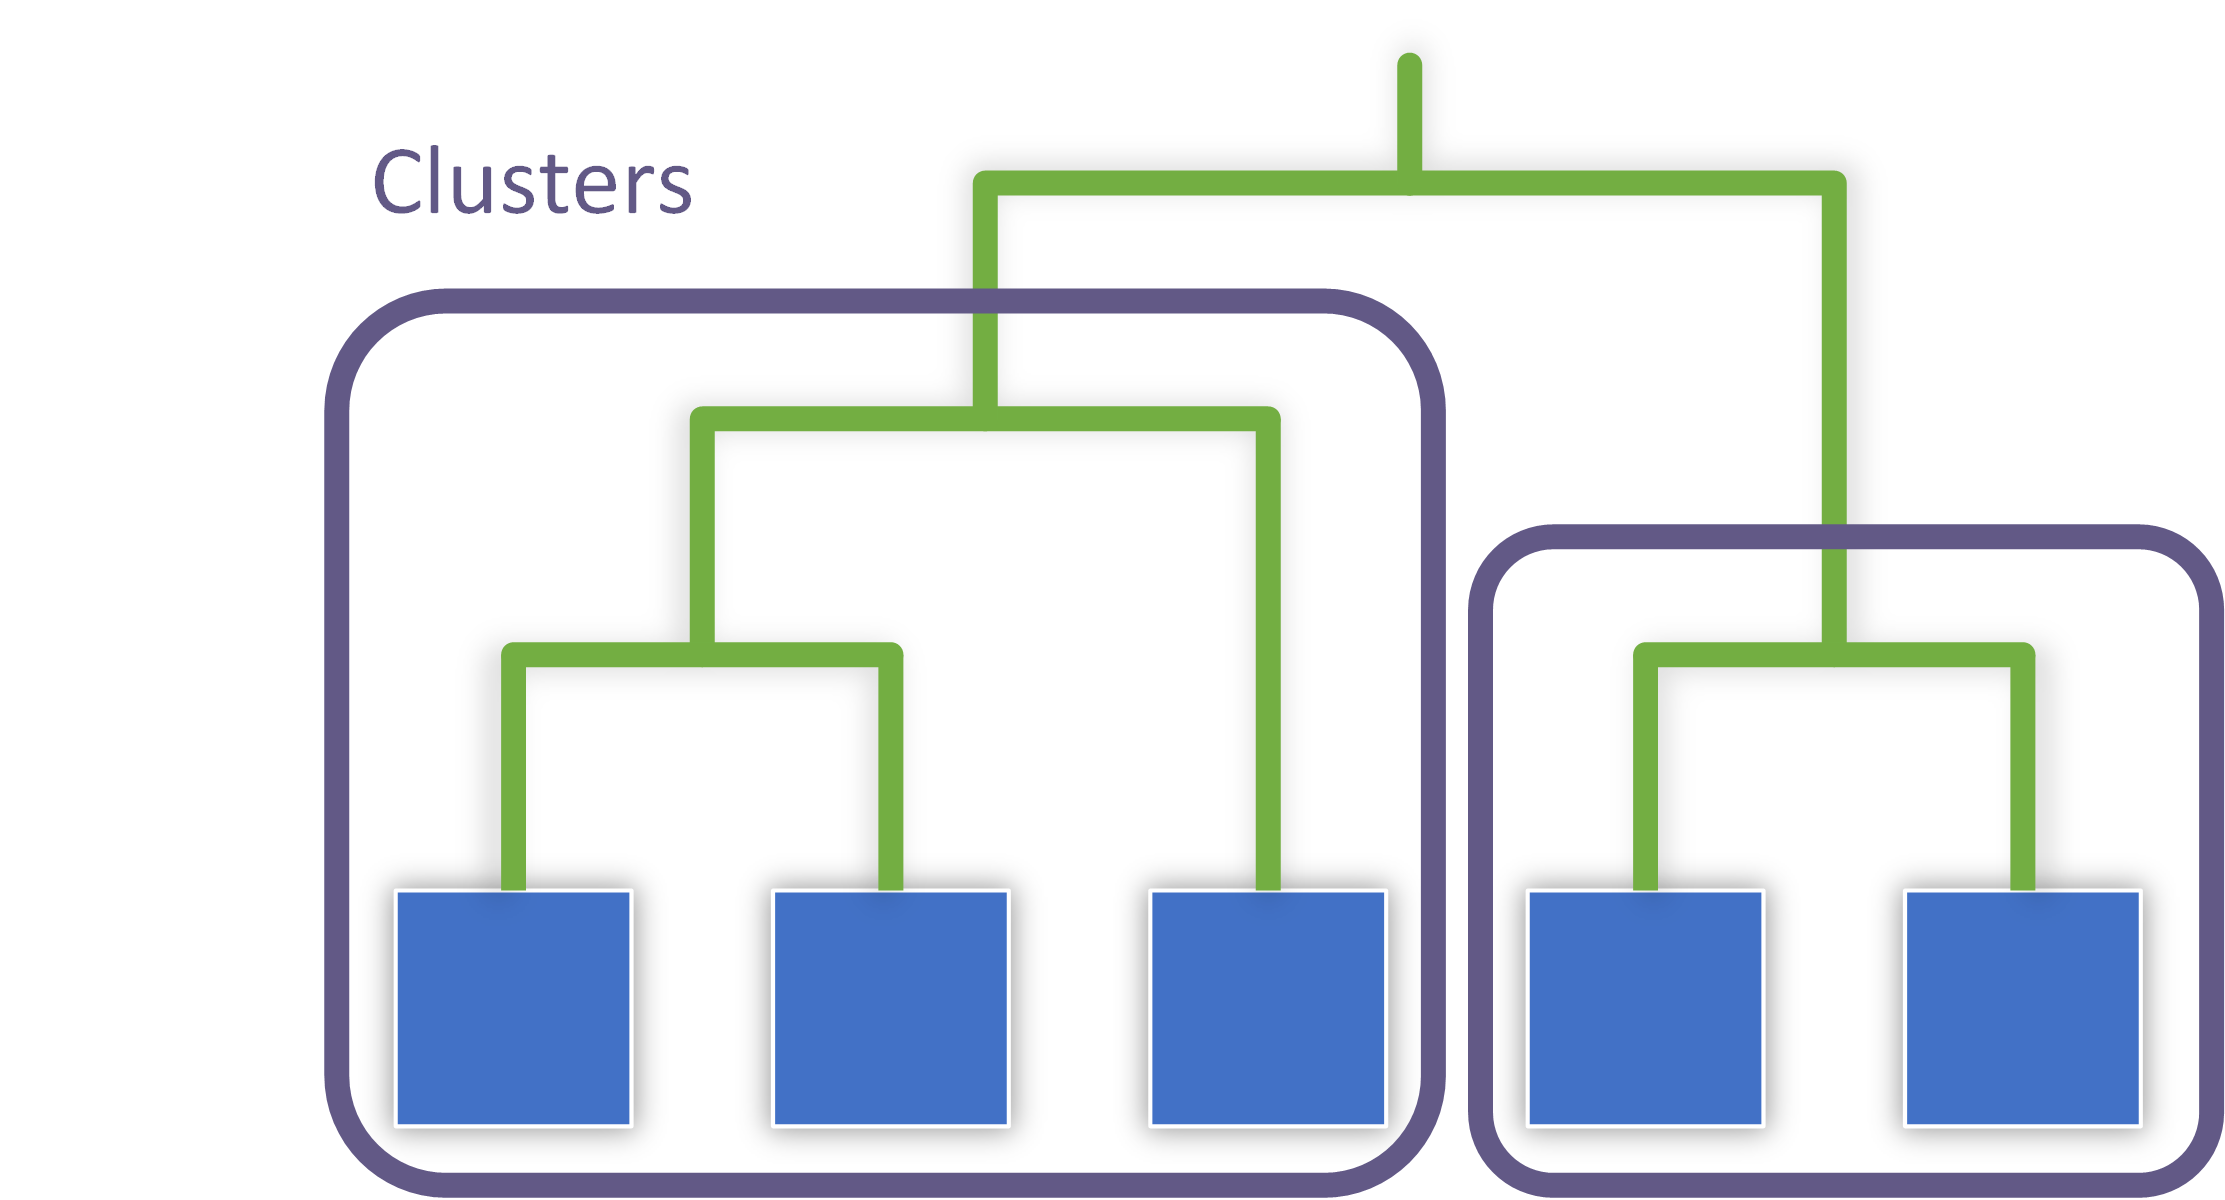
\includegraphics[width=\linewidth]{hierarchy_with_clusters.png}
        \end{mdframed}
        \caption{Example of two clusters created from the hierarchy}
        \label{fig:hierarchy_with_clusters}
    \end{subfigure}
    \caption{Visualisation of the output of hierarchical clustering algorithms}
\end{figure}


\section{Cluster Analysis}
\label{sec:clusterRating}
To evaluate the generated clusters different measurement methods are necessary. Jun. Prof. Dr. Reinhard König from the ETH Zurich proposed the following parameters:

\begin{itemize}
    \item Geometry based measurements:
    \begin{itemize}
        \item Area based on the convex hull of the cluster area
        \item Total length of the streets
        \item Ratio between the area and total length
        \item Distribution variance of the street length
        \item Distribution variance of the street angles
        \item Ratio between street block size and surrounding circle area (minima, maxima, mean)
    \end{itemize}
    \item Centrality-based measurements normalized by the street count (minima, maxima, mean):
    \begin{itemize}
        \item In-Centrality (Integration)
        \item In-Betweenness-Centrality (Choice)
    \end{itemize}
\end{itemize}
The centrality based ratings and the block area calculation were already implemented in \acrshort{acr:CPlan} (section \ref{CPlan}). Additionally a GUI to compare and store the results as JSON-File for each generated cluster has been added.

Some initial measurements and comparisons are made in the cluster analysis chapter \ref{sec:measurements-cluster-analysis}.

\subsection{Block Area Ratio}
In the paper \textit{A typology of street patterns}\citep{blockArea:2014} the method is described how cities/areas can be classified and compared by analysing the block areas instead of the streets. First the block area is calculated and then the result is divided by the circumscribed circle area.

\subsection{Centrality}
The parameter \textit{Integration} describes the closeness centrality. This means the normed sum of the distances from all other vertex based on the shortest path algorithm is calculated. The vertex with the lowest value must be the most central.

With \textit{Choice} the betweenness centrality is described. The approach is to calculate the shortest path between every vertex. Every time a given vertex is visited the betweenness-centrality value of the vertex is raised by one. As a result the highest measured value indicates for a vertex to be in or near the centre of a graph.

\subsection{Variance}
The parameter variance describes the sigma of the normal curve of the distribution function.
First of all the measured data is round to fit into a distribution function (listing \ref{eq:distribution_function}). Then the expected value (listing \ref{eq:expected_value}) and the variance (listing \ref{eq:variance}) is calculated. Finally the standard deviation (square root of V(x)) is computed (listing \ref{eq:standard_deviation}).
\begin{align}
\label{eq:distribution_function} 
F(x) &= P(X \leq x) =  \sum_{t\in{X}, t\leq{x}}{f(t)} \\
\label{eq:expected_value} 
E(x) &= \int\limits_{-\infty}^\infty x \cdot f(x)dx \\
\label{eq:variance} 
V(x) &= \int\limits_{-\infty}^\infty (x - E(X))^2 \cdot f(x)dx \\
\label{eq:standard_deviation} 
\sigma(x) &= \sqrt{V(x)}
\end{align}

\section{All Pairs Shortest Path} \label{sec:shortest_path}
\Gls{APSP} algorithms calculate the shortest path between any two vertices in a graph. A common \acrshort{APSP} algorithm is the algorithm from Floyd and Warshall. It is very simple and directly yields the distance matrix between any two vertices in $O(|V|^3)$ time complexity even if the graph has edges of negative weight.

The \gls{SSSP} algorithm from Dijkstra can also be used as an \acrshort{APSP} when starting a separate run of it from each vertex. A single execution of the Dijkstra algorithm has a worst case performance of $O(|E|+|V|log|V|)$. So the described strategy for \acrshort{APSP} runs in $O(|V||E| + |V|^2 log|V|)$ time complexity. This shows that for graphs with low density this is more performant than Floyd-Warshall. Furthermore the different instances of the algorithm can be executed in parallel. The Dijkstra algorithm does in general only work for graphs with exclusively non-negative edge weights.

%TODO reference?


\FloatBarrier
\chapter{Problem}
The idea of \gls{FCL} is to create, analyse and understand sustainable cities. All tools created for this purpose are provided as open source. The \acrlong{iA} has made many contributions to the \gls{FCL} in recent years. In the course of which CPlan \ref{CPlan} was often used and further developed.

%With CPlan cities can be imported and block areas can be created. Many growing algorithms with random parameter exist and are fully working. To apply modification on the created cities a tree should be created from the existing street network. This would allow genetic modifications on existing networks.

%Random parameters to generate new cities are a good approach but it is not possible to use existing map data. To work with predefined subnetworks of a city map these parts have to be separated based on the given data.



The extracted parts should then be measured for their usefulness to reuse and recombine them at a new position in a new generated city.


\FloatBarrier
\chapter{Concept}
\section{Tree Creation}
To create a tree from an existing graph the angle and distance should be enough data to fully represent a graph.
Two approaches exist to define angles. One is to separate the circle range into minus and plus 180 degrees. This would allow to step straight forward with the angle 0 degree (Figure \ref{fig:tree-generation-decision} left). Another approach is to use the range from 0 to 360 degrees. In this case straight forward would be 180 degrees (Figure \ref{fig:tree-generation-decision} right).

\begin{figure}[!ht]
    \centering
    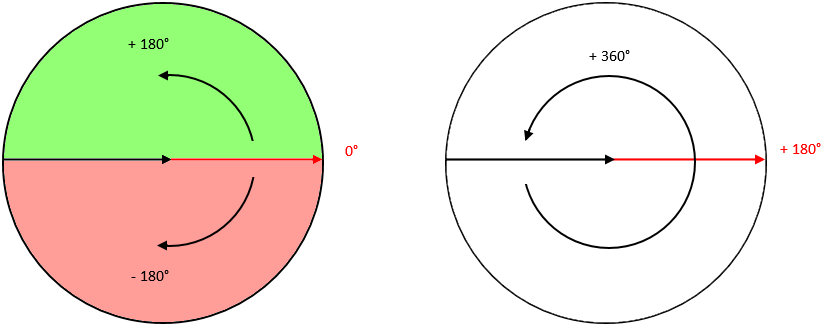
\includegraphics[width=\textwidth]{tree-generation-decision.png}
    \caption{Degree separation \label{fig:tree-generation-decision}}
\end{figure}

Because a tree can not fully represent a graph, many points exist multiple times in the resulting tree. To recreate a graph, junctions should be added where streets intersect without junctions. And the resulting graph should be snapped where points are at the same position. Additionally the existing multiple points in the graph should be removed.

\FloatBarrier
\pagebreak
\section{K-Means}
Points are assigned to different clusters by using the minimal distances. The following approach is used:

\begin{enumerate}
    \item First, random centroids are created.
    \item Then every point is assigned to the nearest centroid by calculating the euclidean distance.
    \item Then centroids are moved to the center of their assigned graph points.
    \item Till no point is moved or the maximum iterations is reached the process is repeated from item 2.
\end{enumerate}

\subsection{Connected Cluster Problem} \label{sec:kmenasProblem}
The K-Mean algorithm is based on the euclidean distance between cluster centroids and street junctions, the edge data (e.g. street length) is not used. As a result it leads to unexpected transitions between clusters.

\subsection{Connected Cluster Approach} \label{sec:connected_cluster_approach}
To solve the problem of unexpected transitions between clusters the best result of the K-Means algorithm can be combined with the distance measurement of a \acrlong{APSP} (\acrshort{APSP}) algorithm (Dijkstra / Floyd-Warshall). These algorithms are used for the hierarchical clustering algorithms \ref{sec:shortest_path}.

\pagebreak
\section{Hierarchical Clustering}
%TODO Short version what singe linkage & PGMA does

\subsection{Hight Memory Usage}
Because WPGMA / UPGMA needs to store all data the memory footprint would be very high. %TODO Describe why exacter.

\subsection{Output Modification}
Idea of output modification
%TODO Describe Idea of output modification!

\pagebreak
\section{Cluster Analysis}
To measure and compare the different areas they should be characterized. Therefore some districts with noticeable characteristics haven been selected an compared to each other. The found characteristics could help to separate a given city on a feature based approach.

%TODO compare corretly only between images not measurements! 

\subsection{Historic District}
\label{sec:historyDistinct}
This district is characterised by a hight count of short streets with many connections. As a result the block areas are small and the block count per area is high. Additionally the mean angles are hight and the density (convex hull area divided by total street length) is low. This characteristics can be observed in the image \ref{fig:historic_district}.

\begin{figure}
    \centering
    \begin{subfigure}[b]{0.6\textwidth}
        \begin{mdframed}[style=mdthight]
            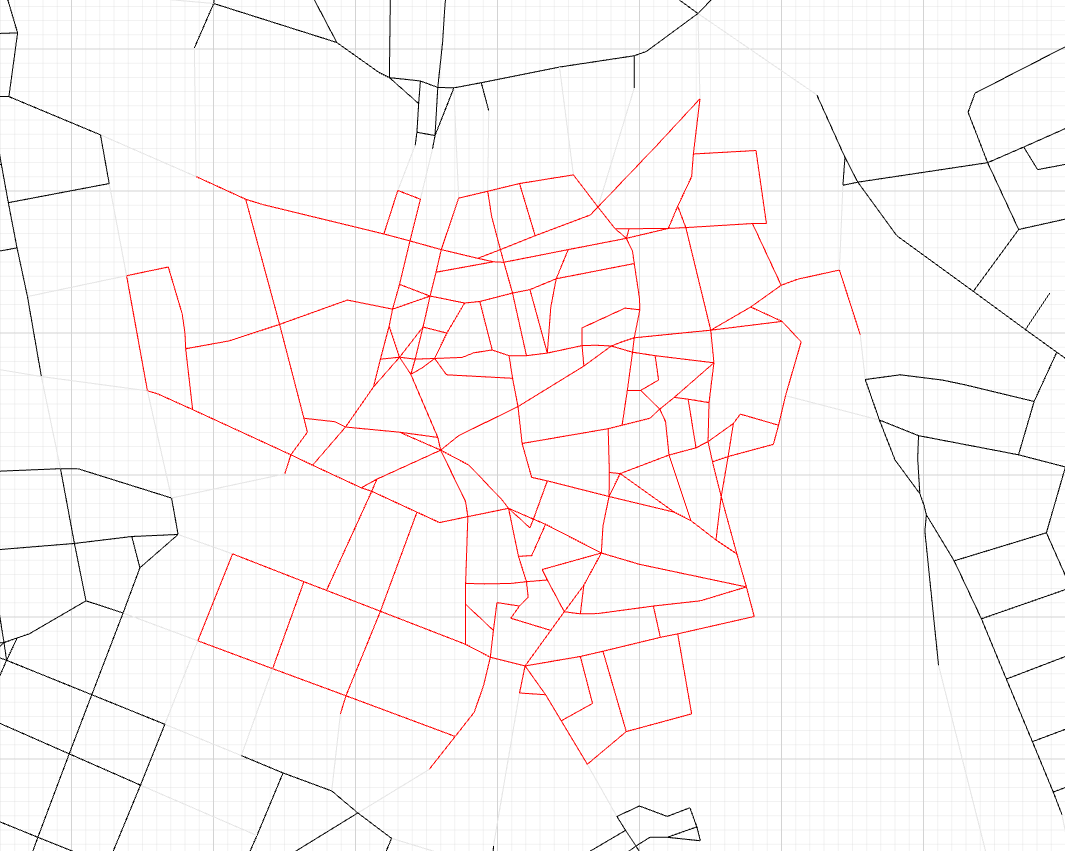
\includegraphics[width=\linewidth]{historic_district.png}
        \end{mdframed}
        \caption{Historic District of Weimar}
        \label{fig:historic_district}
    \end{subfigure}
    \par\medskip
    \begin{subfigure}[b]{0.6\textwidth}
        \begin{mdframed}[style=mdthight]
            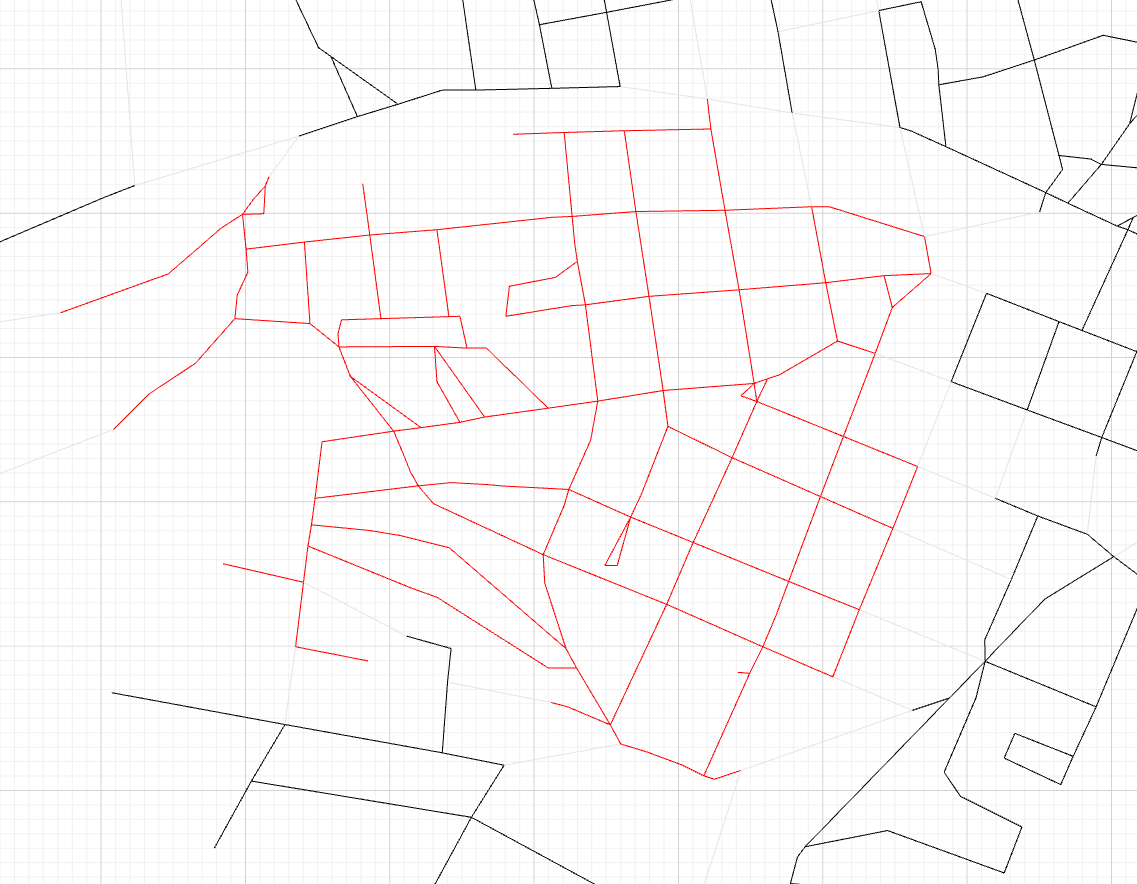
\includegraphics[width=\linewidth]{business_district.png}
        \end{mdframed}
        \caption{Business District of Weimar}
        \label{fig:business_district}
    \end{subfigure}
    \begin{subfigure}[b]{0.6\textwidth}
        \begin{mdframed}[style=mdthight]
            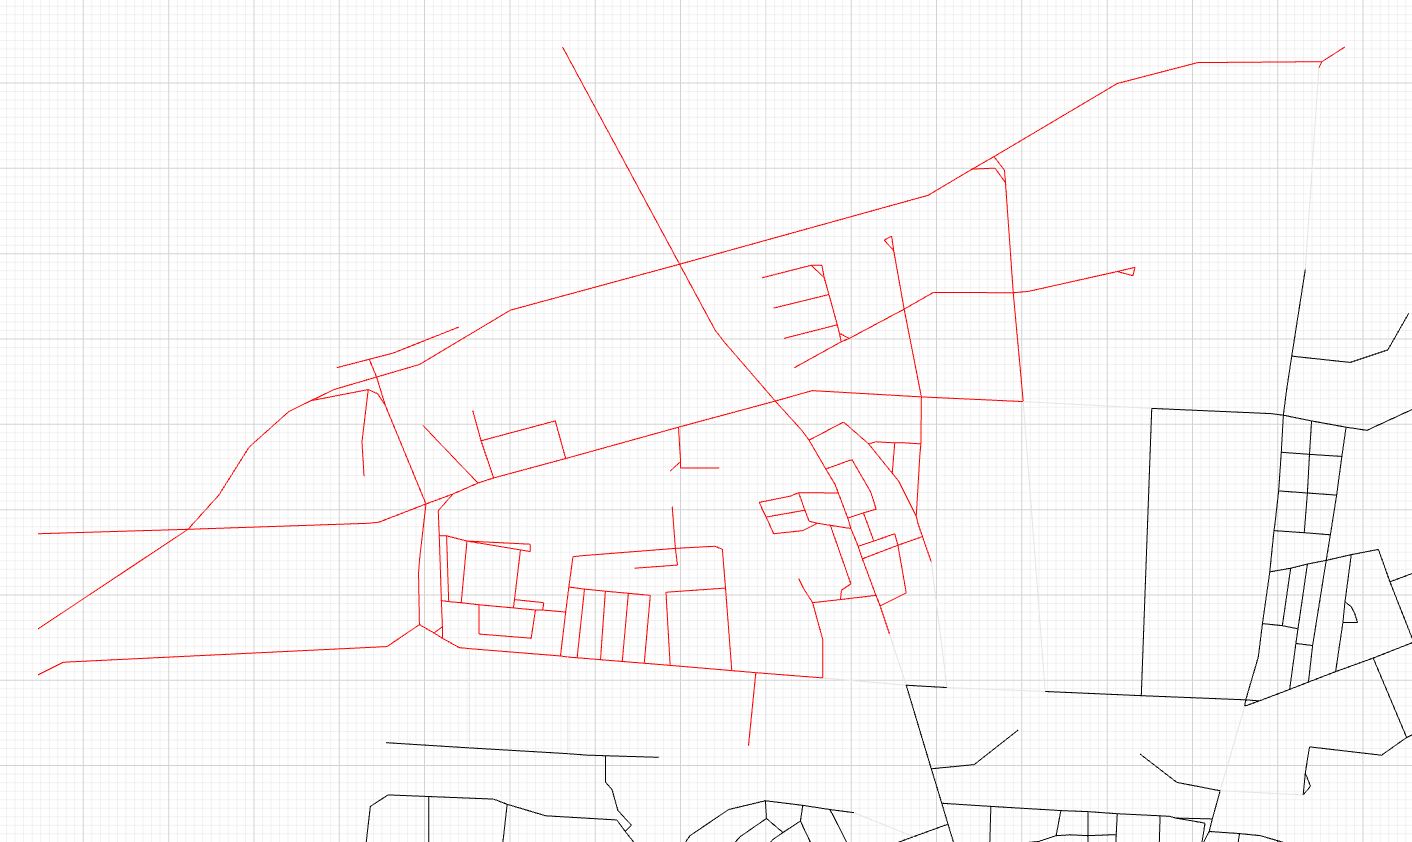
\includegraphics[width=\linewidth]{outskirts_district.png}
        \end{mdframed}
        \caption{Outskirts Area of Weimar}
        \label{fig:outskirts_district}
    \end{subfigure}
    \caption{Different areas of Weimar. Historic District (\ref{fig:historic_district}), Business District (\ref{fig:business_district}) and Outskirts Area (\ref{fig:outskirts_district})}
\end{figure}

\subsection{Business/Manhattan District}
\label{sec:businessDistinct}
If the relative block area (block area divided by surrounding circle) is high the given area is probably a business/Manhattan district. Most of the parameters are in the midrange. The image \ref{fig:business_district} with the measured data in table \ref{sec:ClusterAnalysisMeasurements} in column C2, is an example area of this district/area type.

\subsection{Outskirts Area}
\label{sec:outskits}
These areas are characterized by extreme long streets and a low connection count. As a result the density is extremely high as you can see in the example \ref{fig:outskirts_district} and the measured data in table \ref{sec:ClusterAnalysisMeasurements} in column C3. The block count is compared with a business or historic district exceptional low.

\FloatBarrier
\pagebreak
\chapter{Solutions}
\section{Tree Creation}


\section{K-Means}
To separate street networks the centroid based clustering algorithm K-Mean can be used. The added implementation in CPlan \citep{cPlan:2015} is an optimised K-Means version named K-Means++. The idea of this algorithm is to select reasonable start centres to avoid many iterations.

\subsection{Connected Cluster Implementation} \label{sec:K-Means_shortest_path}
As described in section \ref{sec:connected_cluster_approach} the edge based distances can be calculated with a \acrlong{APSP} (\acrshort{APSP}) algorithm. Based on these distances the cluster points are then assigned. The result is a connected graph. This means every vertex can be reached from every other vertex within a cluster. In the generated figure \ref{fig:Kmeansshortestp} the artefacts described in \ref{sec:kmenasProblem} are removed.

Additional calculation time is needed for the shortest path algorithm. The differences can be compared in the section Measurements \ref{sec:measurements}.

\subsection{Speed Optimization}
The ETH-Zurich provided the following networks: Bad Berka (552 nodes, 626 edges), Weimar (2012 nodes, 2646 edges) and Zurich (27446 nodes, 35121 edges). The network Zurich with factor 13 more edges than Weimar resulted in long processing time. A speed improvement was  achieved by running the K-Means iterations in parallel. Every iteration can be executed free of side effects. The measurements and comparisons of the results are provided in the following section \ref{sec:measurements};

\pagebreak
\section{WPGMA / UPGMA}
\subsection{Memory usage} \label{sec:memory_usage}
The most trivial solution would be to store the distances as a matrix of double-precision floating-point numbers. This is because the given numeric data was already in this number format and a matrix is easily accessible. For \acrshort{UPGMA} and \acrshort{WPGMA} this matrix has to be extended so it also includes the cached distances between clusters.

This storage strategy would use $(2n-1)^2$ double-precision floating-point numbers, $n$ being the node count (number of junctions). As an example: For the used environment this storage strategy would amount to about 21.7 Gigabyte of used memory for the street network of Zurich.

The easiest optimisation is to convert all distances to a single-precision floating-point format. The loss of precision is not affecting the result, as mostly only the $<$ and $>$ relations of the different distances are important.

A second optimisation that can be applied is, to remove redundant information. When storing the full matrix of all distances, most values are stored twice. The matrix is mirrored along the diagonal, because the used street networks are undirected graphs. So the memory usage can almost be cut in half if those duplicates are not stored. This improvement is visualised in figure \ref{fig:memory_usage_01}.

The third and last applied optimisation was to change the way, how cluster distances are stored if the reduction formula \acrshort{UPGMA} or \acrshort{WPGMA} is used. Each time, when two clusters are combined, the distances of the new formed cluster to every other cluster are calculated. This combination step is done using the distances stored for the two old clusters. Afterwards the distances which were stored for the old clusters are no longer used. To reduce the memory usage, the distances of the new cluster can therefore be stored, at the location where the distances of one of the old clusters were stored. Figure \ref{fig:memory_usage_02} visualises this optimisation.

When applying those memory usage optimisations, $\frac{1}{2}n(n+1)$ single-precision floating point numbers have to be stored. The memory complexity still lies in $O(n^2)$, but the improvements allow most modern computers to analyse medium to big sized street networks. As an example: For the used environment the memory usage would amount to about 1.36 Gigabyte for the street network of Zurich.

\begin{figure}
    \centering
    \begin{subfigure}[b]{\textwidth}
        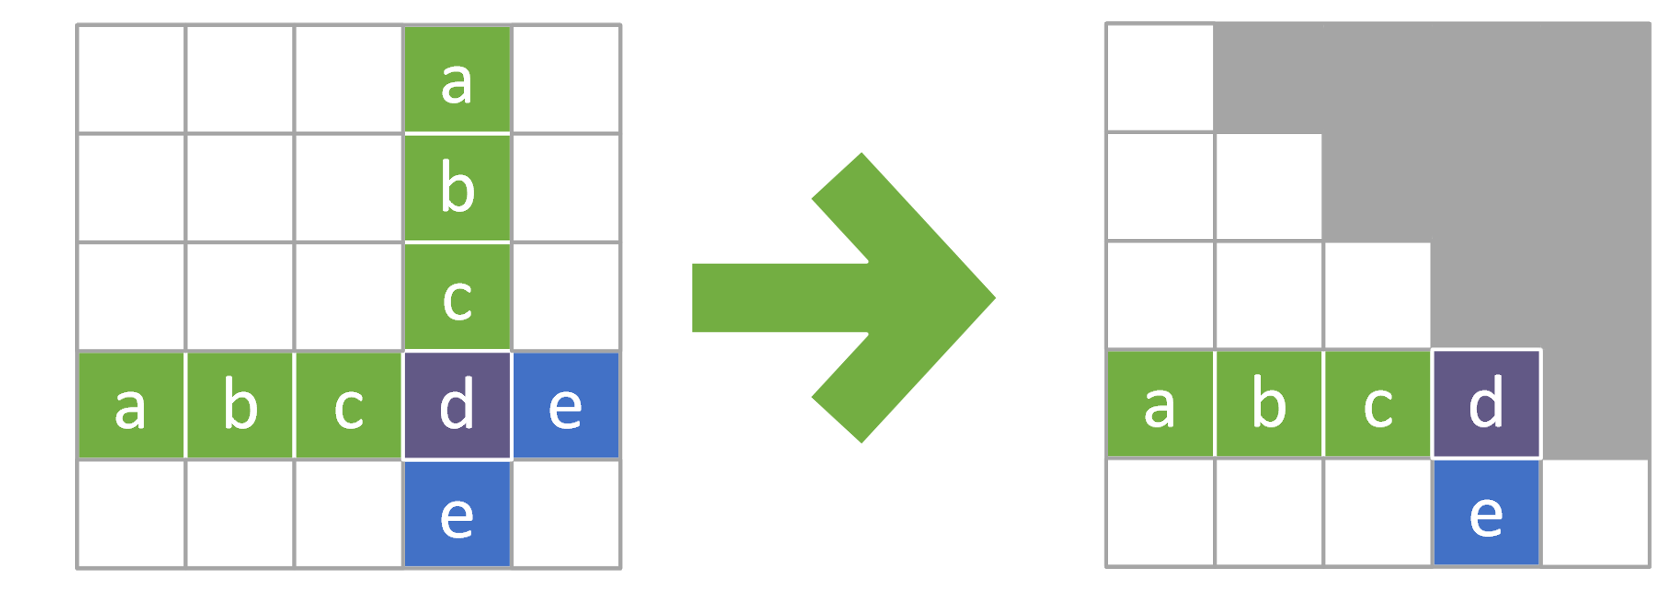
\includegraphics[width=\linewidth]{memoryusage01.png}
        \caption{Optimisation of memory usage by not storing redundant information. On the left hand side is the full distance matrix, on the right hand side is the same matrix without the duplicate entries.}
        \label{fig:memory_usage_01}
    \end{subfigure}
    \par\medskip
    \begin{subfigure}[b]{\textwidth}
        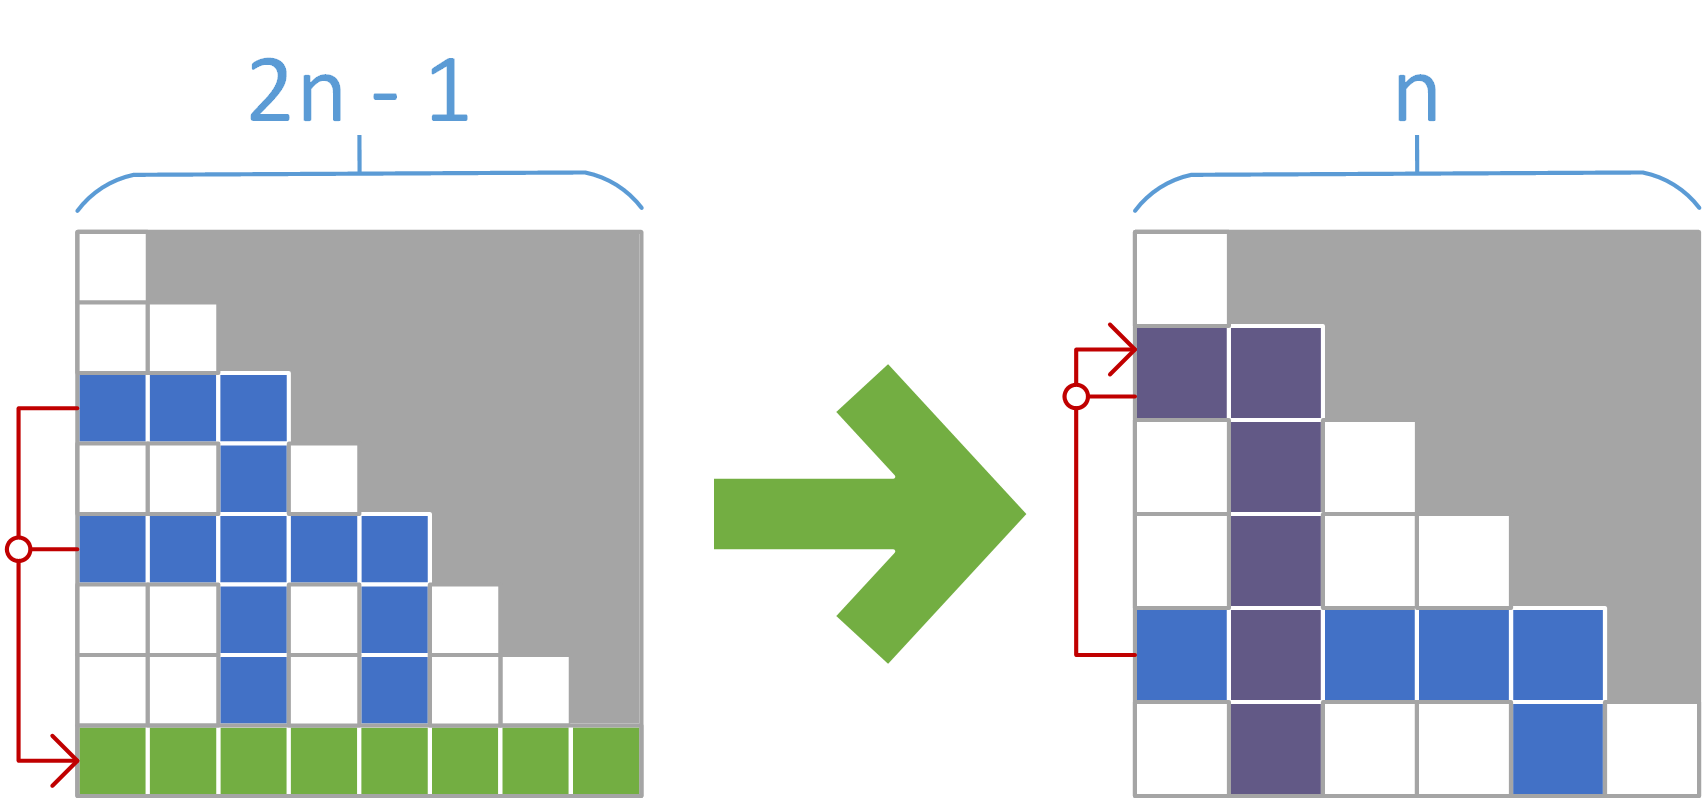
\includegraphics[width=\linewidth]{memoryusage02.png}
        \caption{Optimisation of memory usage by changing the cluster combination behaviour. On the left hand side the blue distances belonging to the old clusters are combined and stored in a new row (of green distances) belonging to the new formed cluster. The right hand side is similar, but the distances of the old clusters (blue and violet) are combined and stored at the location of one of the old clusters (violet). After the combination, the violet distances belong to the new formed cluster.}
        \label{fig:memory_usage_02}
    \end{subfigure}
    \caption{Visualised memory usage optimisations}
\end{figure}

\subsection{Output Modification} \label{sec:outout_modification}
In some cases the hierarchical clustering has an output of clusters with highly varying size if standard splitting order is used. (Size meaning the node / street junction count in this context.) In figure \ref{fig:unmodified_cluster_size} a clustering of Weimar with such a case is shown. In this figure there is a relatively big cluster in the centre of the city and at the bottom left corner are multiple very small clusters.

Depending on the requirements this is the desired result, as this is the optimal solution of the algorithm using the given distances. In other cases it is more important, that the created clusters are of about the same size, than it is to abide the mathematically optimal solution.

To create relatively equally sized clusters from the resulted hierarchy of a hierarchical cluster algorithm the following approach was taken. Instead of splitting the hierarchy into clusters exactly in the order in which the hierarchy was created, the order is changed. When always splitting the biggest cluster (cluster with the most nodes), a result with much more equally sized clusters will be created. A clustering with such modified sizes is shown in figure \ref{fig:modified_cluster_size}.

\begin{figure}
    \centering
    \begin{subfigure}[b]{0.49\textwidth}
        \begin{mdframed}[style=mdthight, userdefinedwidth=0.9\linewidth]
            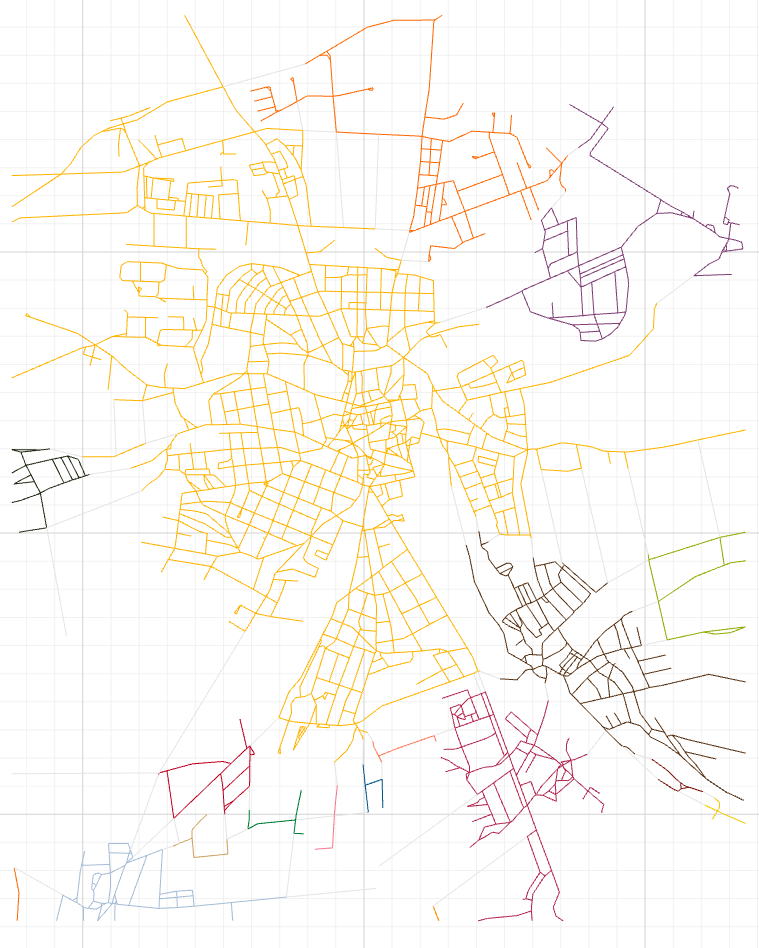
\includegraphics[width=\linewidth]{unmodified_cluster_size.png}
        \end{mdframed}
        \caption{Clusters with original size}
        \label{fig:unmodified_cluster_size}
    \end{subfigure}
    \begin{subfigure}[b]{0.49\textwidth}
        \begin{mdframed}[style=mdthight, userdefinedwidth=0.9\linewidth]
            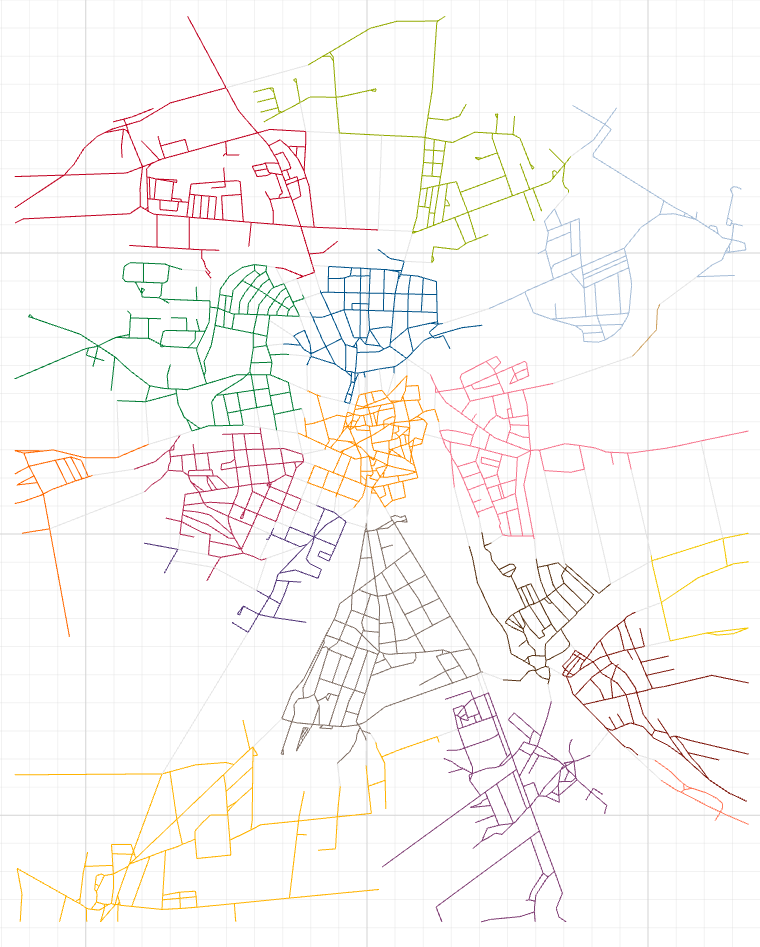
\includegraphics[width=\linewidth]{modified_cluster_size.png}
        \end{mdframed}
        \caption{Clusters with modified size}
        \label{fig:modified_cluster_size}
    \end{subfigure}
    \caption{Clustered street network of Weimar without \ref{fig:unmodified_cluster_size} or with \ref{fig:modified_cluster_size} cluster size modification. (Cluster count = 18, Reduction Formula = \acrshort{UPGMA})}
\end{figure}

\pagebreak
\section{CPlan Improvements}
\begin{itemize}
    \item Some calls to the methods IEnumerable.ToArray() and IEnumerable.ToList() were removed. This method creates a new array / list and stores every item of the IEnumerable in this new collection. As a result the application had an extremely large footprint. To further reduce this overhead some methods were changed to take IEnumerable parameters instead of arrays.
    \item Certain graph and geometry extension methods were fixed. It would be good practice to create unit tests for such methods.
    \item The vector represented by the class Matrix2d is clockwise despite the norm is counter clockwise.
    \item Line intersections of the class Geometry2D was not correct detected an therefore corrected. 
\end{itemize}

\section{Genetic algorithms}
The ETH-Zurich already has genetic optimizations algorithms based on trees. Unfortunately they don't have a working solution to produce a tree from the existing graph. The new created tree generation produces a relative tree with absolute angles. This allowed an easier and faster work process with tree based structures.

\pagebreak
\section{Normalising Street Networks}
While testing clustering algorithms on the street network of Zurich one rough spot of this network was found: Not all streets, which lead to a junction are connected to it. As shown in figure \ref{fig:zuerich_error} floating streets exist (highlighted in purple). No end of any of these highlighted streets is connected to the rest of the street network.

To handle those floating streets a network normalisation method was developed. The normalisation snaps (unites) all junctions and street end points, which are positioned close together, into one common junction. The result of this normalisation is shown in figure \ref{fig:zuerich_fixed}.

\begin{figure}
    \centering
    \begin{subfigure}[b]{0.8\textwidth}
        \begin{mdframed}[style=mdthight]
            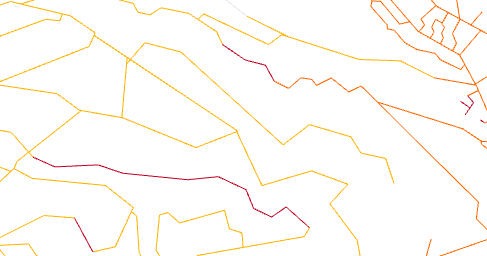
\includegraphics[width=\linewidth]{zuerich_street_error_cropped.png}
        \end{mdframed}
        \caption{Floating streets in the street network of Zurich}
        \label{fig:zuerich_error}
    \end{subfigure}
    \par\medskip
    \begin{subfigure}[b]{0.8\textwidth}
        \begin{mdframed}[style=mdthight]
            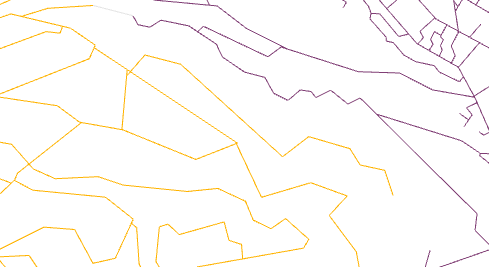
\includegraphics[width=\linewidth]{zuerich_street_fixed_cropped.png}
        \end{mdframed}
        \caption{Normalised street network of Zurich}
        \label{fig:zuerich_fixed}
    \end{subfigure}
    \caption{Street network of Zurich without (\ref{fig:zuerich_error}) and with (\ref{fig:zuerich_fixed}) normalisation}
\end{figure}

\section{Cluster colouring}
To visualize the clustering of a street network in this thesis, clusters are marked with different colours. This section describes the details of this cluster colouring.

The result of each clustering algorithm, which was implemented in this thesis, represents a cluster as set of vertices. Each of these vertices is a junction in the street network. The visualisation only draws streets but not the junctions, as the intersection of streets are intuitively seen as junctions. To colour the different clusters the following approach was taken:

\begin{itemize}
    \item Streets which connect two vertices that are part of the same cluster are coloured with that clusters colour.
    \item Streets which connect vertices of two distinct clusters are coloured grey.
\end{itemize}

There are papers which discuss how colours can be transformed to a perceptually uniform space, where the computation of $n$ colours with maximal distances (for the human eye) is possible \cite{colors:2006}.

In this thesis a more concise approach was taken: The papers of R. M. Boynton \cite{boynton:1989} and K. L. Kelly \cite{kelly:1965} define 11, respectively 22 colours, which are easy to distinguish by human eye. Those colours are displayed in figure \ref{fig:colours}.

Depending on the number of clusters one or the other of those colour sets (without black and white) were used. The colours were already sorted in a way that ensures the extraction of the first $n$ elements returns colours with maximal distance. If more than 20 clusters had to be coloured, the colours of Kelly were used multiple times.

\begin{figure}
    \centering
    \begin{subfigure}[b]{\textwidth}
        \begin{mdframed}[style=mdthight]
            
\includegraphics[width=\linewidth]{boynton_colours.png}
        \end{mdframed}
        \caption{Boynton colours}
        \label{fig:boynton_colours}
    \end{subfigure}
    \par\medskip
    \begin{subfigure}[b]{\textwidth}
        \begin{mdframed}[style=mdthight]
            
\includegraphics[width=\linewidth]{kelly_colours.png}
        \end{mdframed}
        \caption{Kelly colours}
        \label{fig:kelly_colurs}
    \end{subfigure}
    \caption{Colour palette of Boynton (\ref{fig:boynton_colours}) and Kelly (\ref{fig:kelly_colurs})}
    \label{fig:colours}
\end{figure}

\FloatBarrier
\pagebreak
\section{Cluster Analysis}
In CPlan an extension method was implemented for this thesis to directly calculate minimal, maximal, sum and count (mean) on an IEnumerable. This approach allows to directly extract this values without any additional development effort. The following parameters and descriptions characterise all implemented parameter to measure street networks. Additional theoretical information can be found in section \ref{sec:clusterRating}.

\begin{align}
    total\ area &= convex\ hull\ area \\
    total\ length &= street\ length\ sum \\
    density &=\ 'total\ area'\ divided\ by\ 'total\ length' \\
    street\ length\ median &= Middle\ of\ the\ street\ length\ dataset \\
    street\ length\ variance &= \sigma\ of\ the\ normal\ distribution\ curve\ of\ the\ variance \\
    vertex\ connections &= mean\ connected\ edges\ per\ vertex \\
    street\ angle &= angles\ between\ all\ edges\ at\ a\ vertex \\
    street\ angle\ variance &= \sigma\ of\ the\ normal\ distribution\ curve\ of\ the\ angles \\
    block\ count &= total\ block\ count \\
    block\ area\ A/Ac &= block\ area\ divided\ to\ a\ minimal\ circle\ around\ a\ block \\
    integration &= normalised\ in-centrality \\
    choice &= normalised\ in-betweenness-centrality 
\end{align}


\FloatBarrier
\pagebreak
\chapter{Results}
\section{Tree Creation}
A tree is generated from a certain area. To display and compare the differences a graph recreation algorithm was written. Therefore the printed result is also a nearly equal graph. Figure \ref{fig:tree_example} is a selected cluster before the tree creation. Figure \ref{fig:tree_example_after} is the recreated graph from the tree. The grid behind the recreated subgraph is rotated. This rotation depends on the angle of the start edge.

\begin{figure}[hb]
    \centering
    \begin{subfigure}[b]{0.5\textwidth}
        \begin{mdframed}[style=mdthight]
            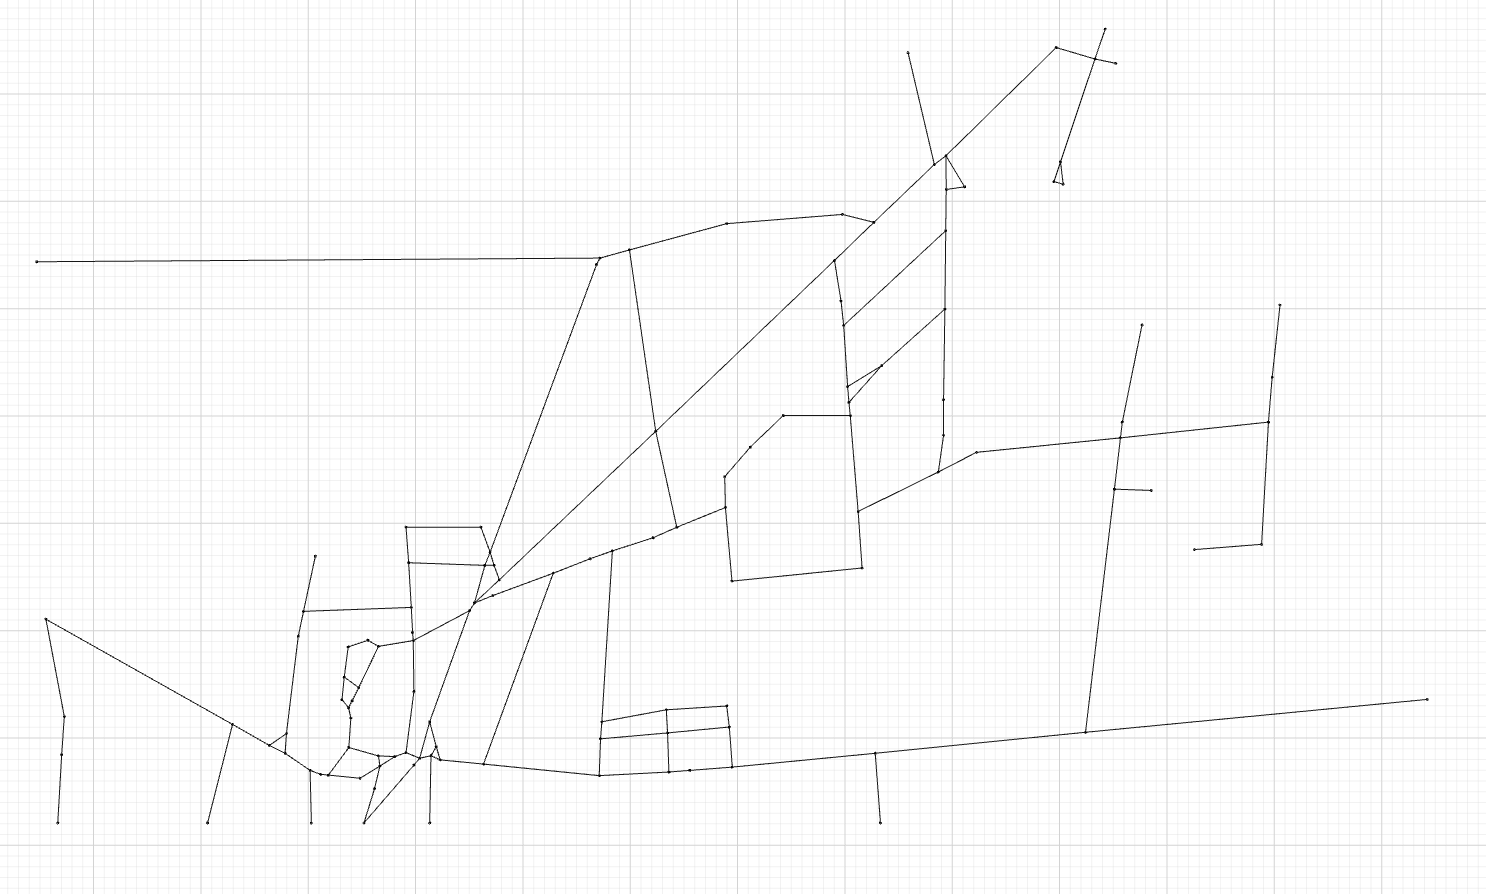
\includegraphics[width=\textwidth]{tree_before.png}
        \end{mdframed}
        \caption{Subgraph of Weimar}
        \label{fig:tree_example}
    \end{subfigure}
    \quad
    \begin{subfigure}[b]{0.5\textwidth}
        \begin{mdframed}[style=mdthight]
            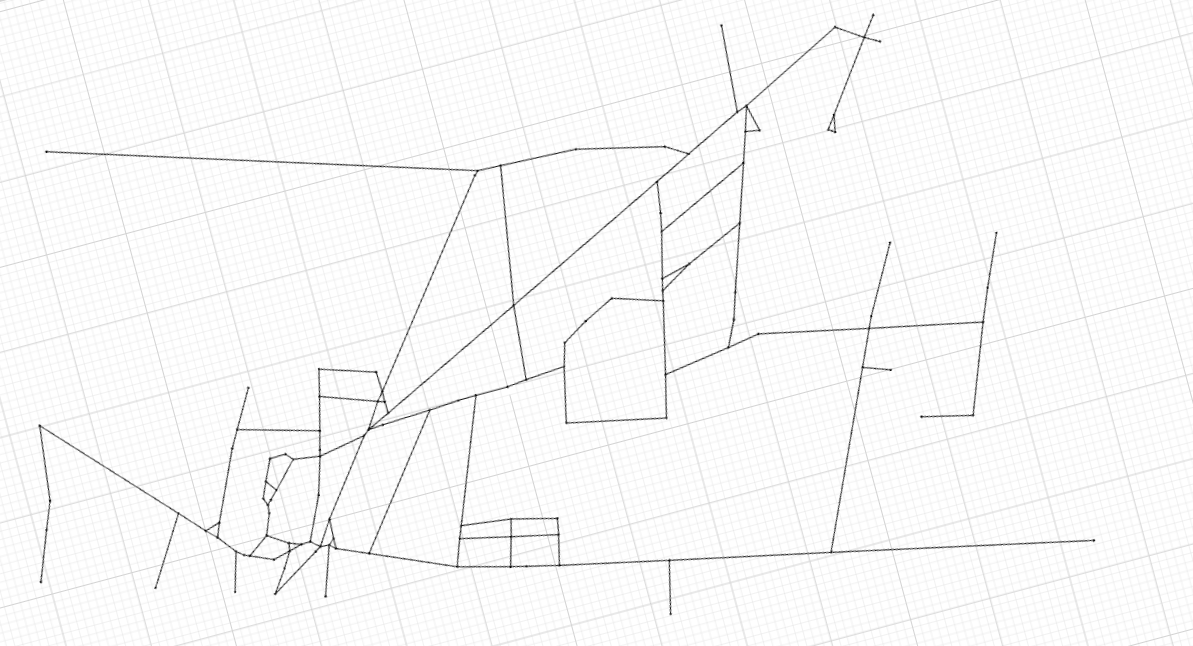
\includegraphics[width=\textwidth]{tree_after.png}
        \end{mdframed}
        \caption{Recreated Subgraph from tree of Weimar}
        \label{fig:tree_example_after}
    \end{subfigure}
    \caption{Subgraph before \ref{fig:tree_example} and after \ref{fig:tree_example_after} tree creation}
\end{figure}

\FloatBarrier
\section{K-Means}
The K-Means algorithm assigns points by using random centroids and assign all nearest points to them. Then the centroids are moved into the centre of their assigned points. This process is repeated till no point is moved.

The implementation in CPlan \ref{CPlan} produced the following image \ref{fig:KmeansGenerated} based on the city of Weimar. All streets in one cluster are marked with the same colour, the transitions between clusters are marked black.

\subsection{Connected Cluster Problem}
As presumed the resulting subgraph had unexpected transitions between clusters. This means some clusters were not connected. In the image \ref{fig:KmeansProblem} the result can be observed in the read circle where only one point is marked as outer cluster. The two black lines represent the cluster transitions.

\begin{figure}[!ht]
    \centering
    \begin{mdframed}[style=mdthight, userdefinedwidth=0.55\textwidth, align=center]
        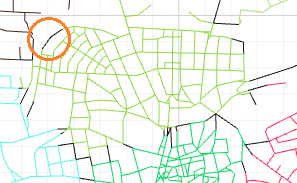
\includegraphics[width=\textwidth]{clusteranalysis_kmeans_problem.png}
    \end{mdframed}
    \caption{Problem of K-Means clustering
        \label{fig:KmeansProblem}}
\end{figure}

\subsection{Connected Cluster Results} \label{sec:K-Means_shortest_path}
To problem was then solved by using a \gls{APSP} algorithm like Dijkstra or Floyd-Warshall. In the following figure \ref{fig:Kmeansshortestp} every cluster is a connected subgraph.

\begin{figure}
    \centering
    \begin{mdframed}[style=mdthight]
        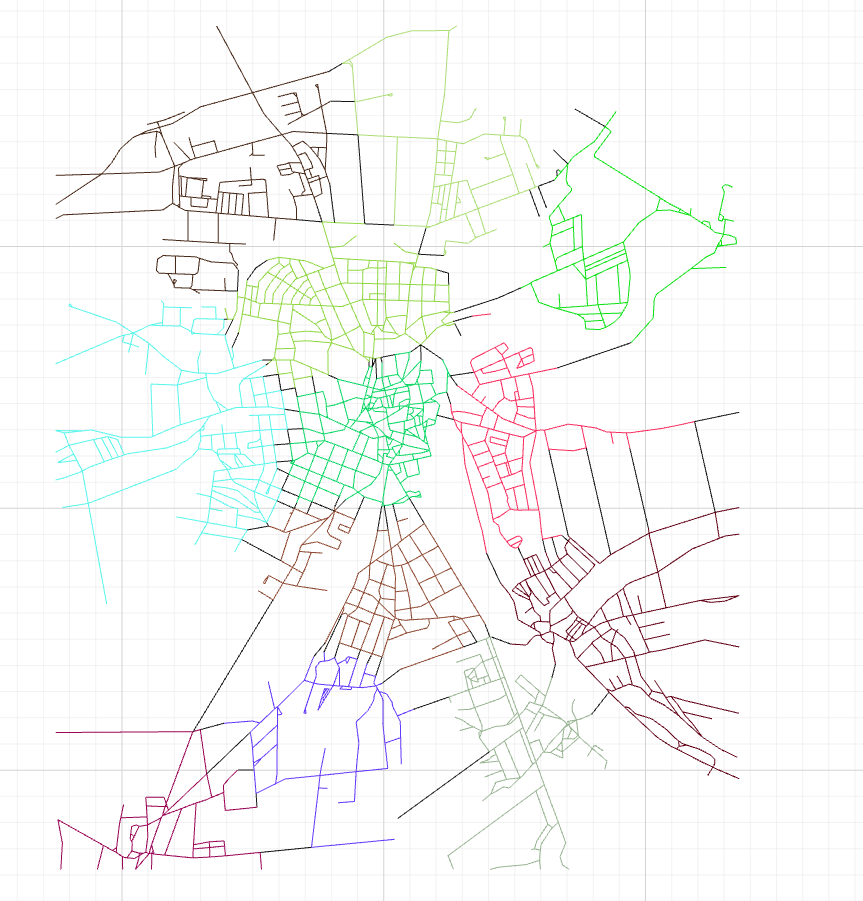
\includegraphics[width=\textwidth]{clusteranalysis_kmeans_result.png}
    \end{mdframed}
    \caption{K-Means cluster analysis of Weimar \label{fig:KmeansGenerated}}
\end{figure}

\begin{figure}
    \centering
    \begin{mdframed}[style=mdthight]
        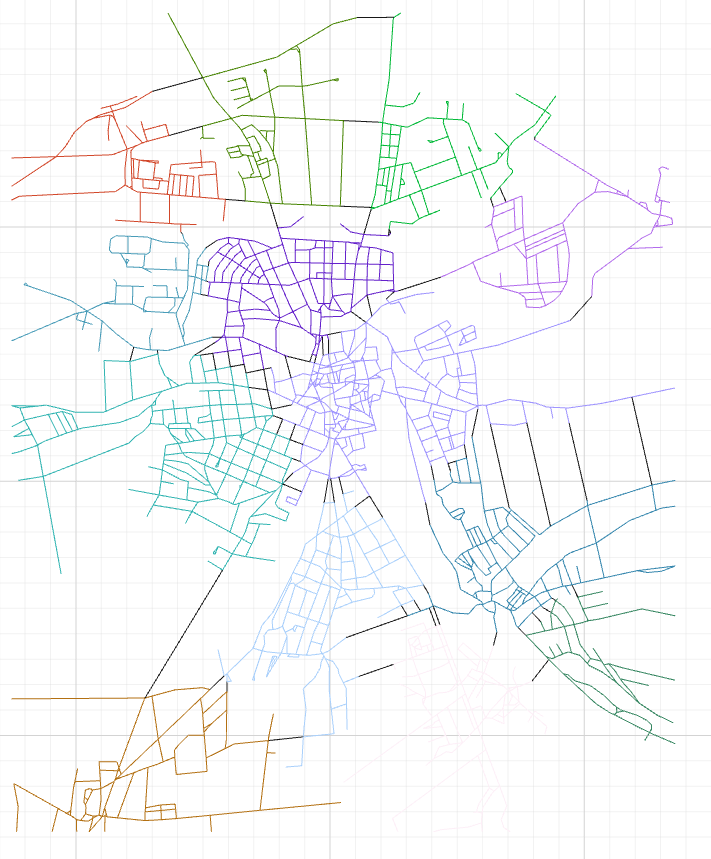
\includegraphics[width=\textwidth]{clusteranalysis_kmeansExt_result.png}
    \end{mdframed}
    \caption{K-Means clustering with shortest path\label{fig:Kmeansshortestp}}
\end{figure}

\section{Single-Linkage Result}
The figure \ref{fig:SingleLinkage} shows the result of a hierarchical cluster analysis of Weimar using the single linkage reduction formula. The used distance function $d(i, j)$ was the shortest distance from $i$ to $j$ in the street graph. As it is clearly visible when looking at the result, this way of cluster analysis is not creating the desired output. There is one huge cluster in the middle and many one-node clusters at the border of the city.

The problem is caused by the used reduction formula. Single linkage uses the minimal distance between all nodes of the compared clusters. This leads to the creation of clusters, where all roads which connect two clusters are long. In a city, where there are multiple (direct and indirect) connections from one junction to another most of the time, this tends to create one-node clusters for nodes, which are connected to the city by a single long road.

\begin{figure}
    \centering
    \begin{mdframed}[style=mdthight]
        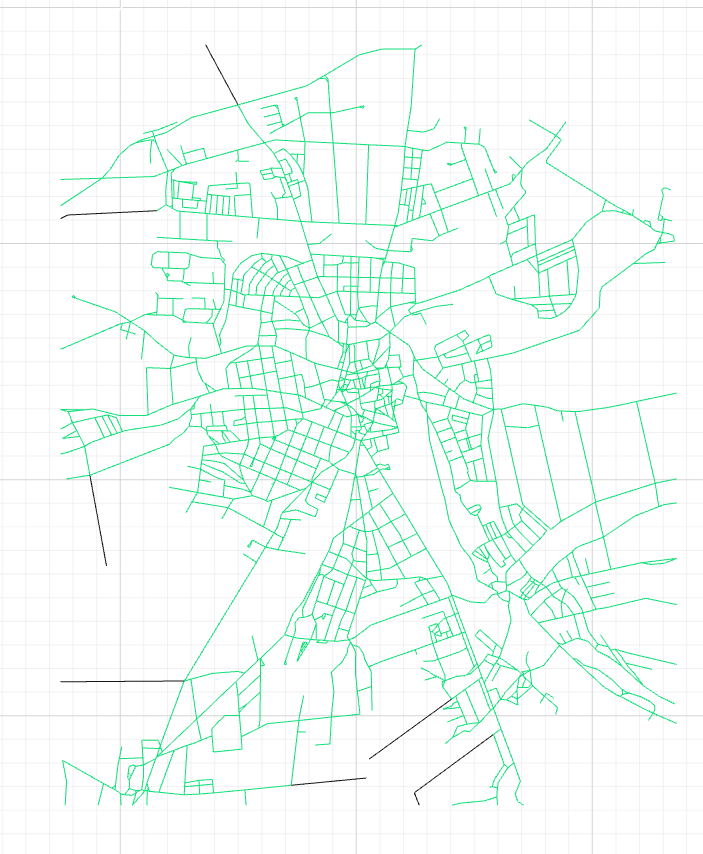
\includegraphics[width=\textwidth]{clusteranalysis_singlelinkage.png}
    \end{mdframed}
    \caption{Single-Linkage hierarchical cluster analysis of Weimar\label{fig:SingleLinkage}}
\end{figure}

\section{UPGMA and WPGMA Result}
\label{sec:UPGMAandWPGMA}
The figures \ref{fig:hierarchical_clustering_upgma} and \ref{fig:hierarchical_clustering_wpgma} show the result of hierarchical cluster analysis using the \acrshort{UPGMA}, or respectively the \acrshort{WPGMA} reduction formula. The same distance function $d(i, j)$ as in the single linkage solution was used (shortest distance from $i$ to $j$ in the street graph).

%TODO: Compare, conclusions?

\begin{figure}
    \centering
    \begin{mdframed}[style=mdthight]
        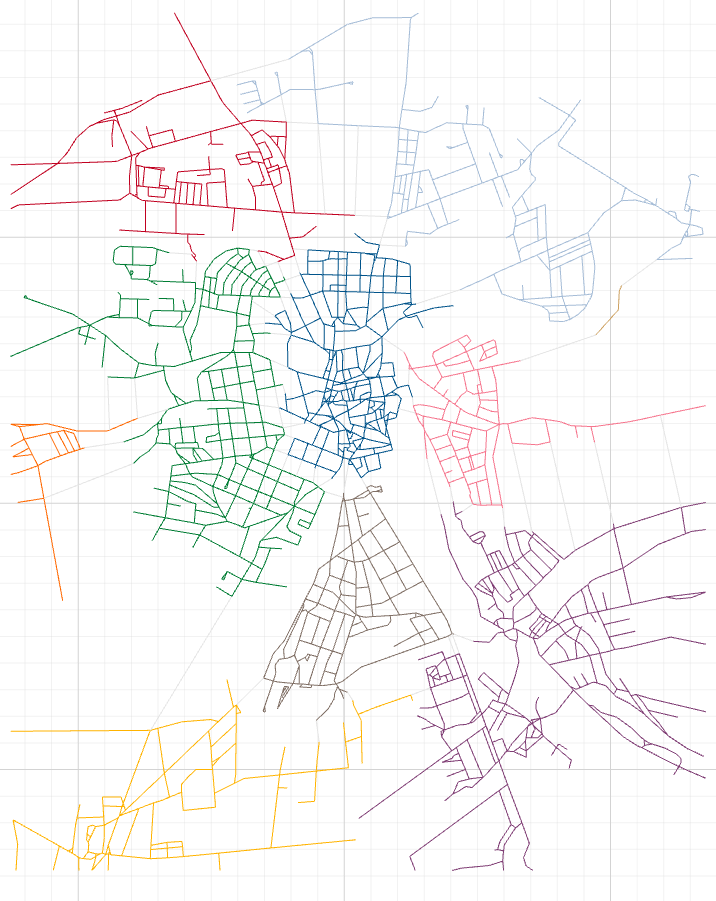
\includegraphics[width=\textwidth]{hierarchical_clustering_upgma.png}
    \end{mdframed}
    \caption{UPGMA hierarchical cluster analysis of Weimar\label{fig:hierarchical_clustering_upgma}}
\end{figure}


\begin{figure}
    \centering
    \begin{mdframed}[style=mdthight]
        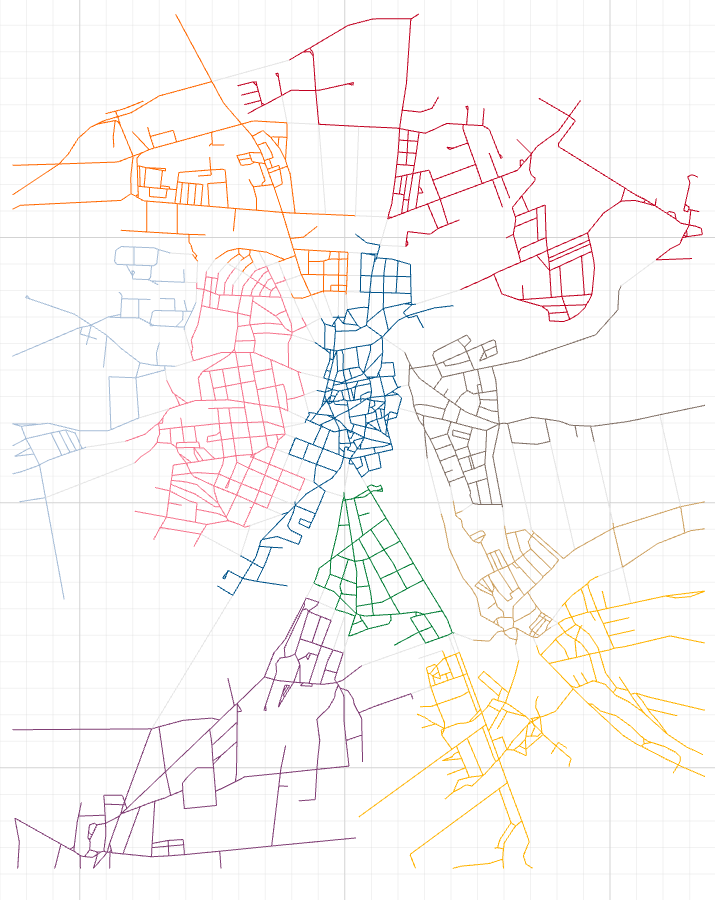
\includegraphics[width=\textwidth]{hierarchical_clustering_wpgma.png}
    \end{mdframed}
    \caption{WPGMA hierarchical cluster analysis of Weimar\label{fig:hierarchical_clustering_wpgma}}
\end{figure}


\pagebreak
\FloatBarrier
\section{Speed Measurements} \label{sec:measurements-speed}
In this chapter the generated data with CPlan \ref{CPlan} is compared and analysed.

\begin{figure}
    \centering
    \begin{mdframed}[style=mdthight]
        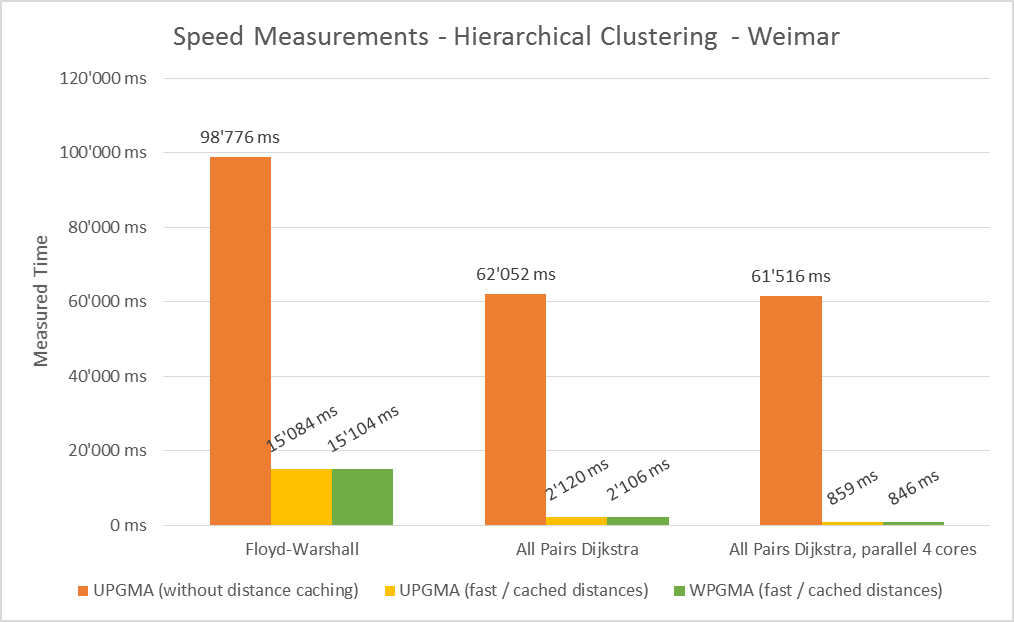
\includegraphics[width=\textwidth]{hierarchical_clustering_speed.png}
    \end{mdframed}
    \caption{\label{fig:hierarchical_clustering_speed}}
\end{figure}

\begin{figure}
    \centering
    \begin{mdframed}[style=mdthight]
        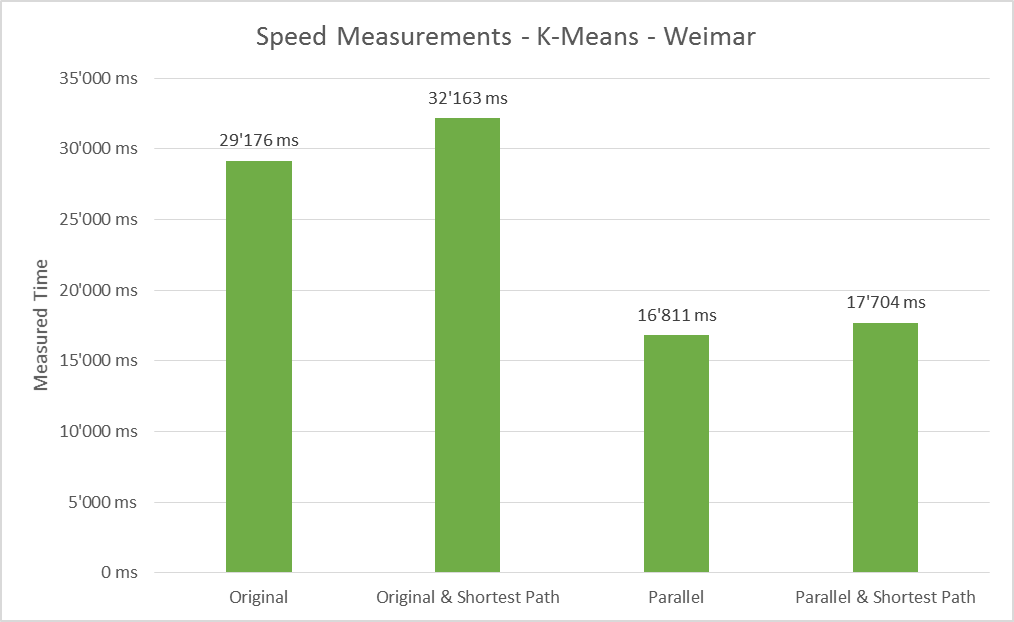
\includegraphics[width=\textwidth]{kmeans_speed.png}
    \end{mdframed}
    \caption{\label{fig:kmeans_speed}}
\end{figure}

TODO: Description of speed measurements here. 

TODO: Table of speed measurements here.

\section{Cluster Analysis}
\label{sec:measurements-cluster-analysis}
In this chapter the provided measurement methods \ref{sec:clusterRating} are used to compare different districts/areas. The following images were generated with the cluster algorithm FastUPGMA \ref{sec:UPGMAandWPGMA} on Weimar with \textit{Modified Output} and \textit{Number of Clusters} count 16.

\subsection{Measured Data}
\label{sec:ClusterAnalysisMeasurements}
The following table \ref{tab:cluterAnalysisDescription} contains the parameters with additional descriptions. Extended information can be found below the table. Of every parameter the minimal (min), maximal (max), mean (average) and the median value can be calculated.

\begin{table}[h]
\begin{center}
    \begin{tabular}{ | l | l |} \hline 
        \textbf{Parameter} & \textbf{Description} \\
        \hline
        Total Area &  Area of the convex hull \\ \hline
        Total Length & Sum of the street length \\ \hline
        Density & 'Total Area' divided by 'Total Length'  \\ \hline
        
        Street Length Min/Max/Mean & Shortest/Longest/Average street length  \\ \hline
        Street Length Median & Middle value of the length dataset \\ \hline
        Street Length Variance & Sigma of the normal distribution curve of the variance \\ \hline
        
        Vertex Connections & Mean connected edges per vertex  \\ \hline
        
        Street Angle Min/Max/Mean & Smallest/Biggest/Average angle between two edges \\ \hline
        Street Angle Variance & Sigma of the normal distribution curve of the angles \\ \hline
        
        Block Count & Total number of blocks \\ \hline
        Block Area Min/Max/Mean & Shortest/Biggest/Average block area \\ \hline
        Block Area A/Ac Min/Max/Mean & Block area divided to a minimal circle around a block \\ \hline
        
        Integration Min/Max/Mean & Normalised In-Centrality \\ \hline
        Choice Min/Max/Mean & Normalised In-Betweenness-Centrality \\ \hline
    \end{tabular}
    \caption{Parameter with descriptions for table \ref{tab:measured_cluster_ratings}}
    \label{tab:cluterAnalysisDescription}
\end{center}
\end{table}


\begin{table}[h]
\begin{center}
\begin{tabular}{ |l|l|l|l|l| }
    \hline
    \textbf{Parmate}r &
    & \textbf{C1} \ref{sec:historyDistinct}
    & \textbf{C2} \ref{sec:businessDistinct}
    & \textbf{C3} \ref{sec:outskits}  \\ 
    \hline
    \multirow{4}{*}{Total} 
    & Area & 1838.05 & 1956.59 & 7802.74 \\
    & Length & 806.92 & 643.50 & 1069.81 \\
    & Density & 2.28 & 3.04 & 7.29 \\
    \hline
    \multirow{5}{*}{Street Length}
    & Min & 0.66 & 0.69 & 0.73 \\
    & Max & 9.13 & 10.68 & 38.00 \\
    & Mean & 2.72 & 3.85 & 4.82 \\
    & Median & 2.30 & 3.65 & 3.28 \\
    & Variance & 1.70 & 2.19 & 5.00 \\
    \hline
    \multirow{1}{*}{Vertex} 
    & Connections & 3.04 & 2.84 & 2.45 \\
    \hline
    \multirow{5}{*}{Street Angle} 
    & Min & 0.00 & 0.00 & 0.00 \\
    & Max & 151.80 & 358.84 & 359.80 \\
    & Mean & 119.03 & 123.75 & 137.18 \\
    & Variance & 124.68 & 131.65 & 129.47 \\
    \hline
    \multirow{5}{*}{Block} 
    & Count & 55 & 35 & 26 \\
    & Area Min & 0.01 & 0.09 & 0.00 \\
    & Area Max & 31.75 & 42.29 & 567.26 \\
    & Area Mean & 6.54 & 13.65 & 76.30 \\
    & A/Ac Min & 0.01 & 0.01 & 0.00 \\
    & A/Ac Max & 0.54 & 0.55 & 0.66 \\
    & A/Ac Mean & 0.18 & 0.23 & 0.18 \\
    \hline
    \multirow{5}{*}{Integration} 
    & Min & 0.46 & 0.48 & 0.60 \\
    & Max & 0.57 & 0.75 & 1.0 \\
    & Mean & 0.49 & 0.59 & 0.78 \\
    \hline
    \multirow{5}{*}{Choice}
    & Min & 0.00 & 0.00 & 0.00 \\
    & Max & 1.00 & 0.67 & 0.34 \\
    & Mean & 0.10 & 0.05 & 0.04 \\
    \hline
\end{tabular}
\caption{Measured results from Historic District (C1) \ref{sec:historyDistinct}, Business District (C2) \ref{sec:businessDistinct}, Outskirts Area (C3) \ref{sec:outskits} and (C4)}
\label{tab:measured_cluster_ratings}
\end{center}
\end{table}


\pagebreak
\FloatBarrier
\chapter{Future Work}
\label{sec:future_work}

Despite many cluster analysis approaches were tested in this thesis, other methods like distribution-based or density-based clustering exist. They could be tested and compared against the implemented versions for this thesis.

Additional features could be used to analyse the given street networks. For example the hierarchy created for the hierarchical clustering method could be used in K-Means or the edge centres could be used instead of the vertices.

To generate faster results some optimisations are possible. For the K-Means algorithm a K-D tree could be used. The current Single-Linkage algorithm $O(n^2)$ could be optimised with a data structure called quadtree to run in time complexity of $O(n)$.

More detailed analysis of the measured clusters could be created based on urban planning data. Additional more detailed measurement methods could be added and the created results compared.

At the \gls{iA} there are other running projects to extend \gls{acr:CPlan} with more functionality. One project is to allow removing a subgraph within a city and grow a new district into the gap starting from the edges. Another project is to recombine the created clusters and use genetic algorithms to grow new cities.

\acrshort{acr:CPlan} was recently ported to a 64 bit architecture. Unfortunately, some libraries are still only 32 bit versions, which leads therefore to problems. For this thesis unit tests were added to \acrshort{acr:CPlan} to ensure the proper working of the new classes and functions. Additionally many tests should be added to test the core functionality of \acrshort{acr:CPlan}. A rework of the application would allow a more efficient and faster development.


\pagebreak
\FloatBarrier
\chapter{Conclusion}
In this thesis different cluster analysis algorithms were compared and extended on a graph representation of a street networks.

The centroid based K-Means algorithm \ref{sec:K-Means} produced reasonable clusters, unfortunately with wrong assignments. Because the assignments were vertex based not every cluster was connected. To correct this error a shortest path algorithm was used \ref{sec:K-Means_shortest_path} to get connected clusters.

For hierarchical algorithms \ref{sec:hierarchicalClustering} there are many different reduction formula algorithms. First the Single Linkage algorithm produced one huge cluster in the middle and many at the border. This algorithm used the minimal distances of all nodes of the compared clusters and therefore in a city with multiple connections one big cluster in the middle was created.

Then the reduction algorithms WPGMA (Weighted Pair Group Method with Arithmetic mean) calculates the average distances between two clusters. The result was many clusters with different sizes. To resolve this issue the UPGMA (Unweighted PGMA) algorithm was tested where all distances are equal. The result was better but the cluster size differences were still too big.

To produce cluster with equal sizes the output was then modified. This means instead of splitting the hierarchy as it was created always the biggest cluster (with the most notes) was split. The modification leads to better balanced clusters as preferred in city clustering.

During tests with big street networks high memory usage was a problems. As a result three optimisations were made \ref{sec:memory_usage}. First, float precision was used. Second, a data structure which does not store value twice was developed. Third the resulting cluster distances were saved at the position of the resource positions.

To rate the created clusters many graph analysis parameters were implemented \ref{sec:measurements}. The values can be compared and exported into a JSON-file for later use.

\bibliography{quotations}
\appendix
\printnoidxglossaries

\appendix
\chapter{Applied in CPlan}
\section{K-Means Clustering Options}
To apply centroid based clustering to a street network a specialized gui dialog was created where all parameters can be set. As you can see in figure \ref{fig:applied_k-means_GUI}.
\begin{itemize}
    \item If 'Show Visualisation' is activated the clustering process will be visualized.
    \item The counter 'Number of Tries' represents the count how often the clustering algorithm will be executed to extract the best result.
    \item 'Iterations per Try' describe how many iterations are maximal made per try. 
    \item If 'Shortest Path' is selected a shortest path algorithm will be applied after the centroid were set.
\end{itemize}
\begin{figure}[ht]
    \centering
    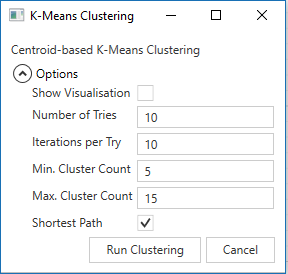
\includegraphics[width=0.47\linewidth]{k-means_clustering_applied.png}
    \caption{This gui dialog represents the parameters which could be applied to the K-Mean clustering algorithm.}
    \label{fig:applied_k-means_GUI}
\end{figure}

\section{Hierarchical Clustering Options}
A specialized gui was created to set parameters for the hierarchical clustering analysis. The reduction formula can be selected at the top \ref{fig:applied_HC_clustering_GUI}.
\begin{itemize}
    \item If the option 'Show Slider Dialog' is selected the cluster count can be changed in an additional dialog \ref{fig:applied_HC_clustering_slider_GUI}.
    \item The field 'Number of Clusters' represents the number of clusters which will be generated.
    \item If 'Modify Output' is selected always the biggest cluster will be split instead as the hierarchy was created.
\end{itemize}

\begin{figure}[ht]
    \centering
    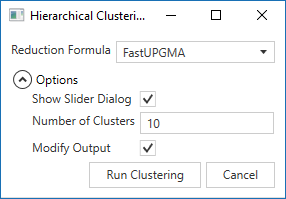
\includegraphics[width=0.47\linewidth]{HC_clustering_applied.png}
    \caption{This gui dialog represents the parameters which could be applied to the hierarchical clustering algorithm.}
    \label{fig:applied_HC_clustering_GUI}
\end{figure}

\begin{figure}[ht]
    \centering
    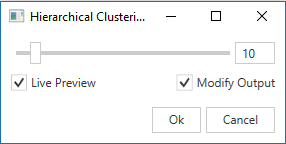
\includegraphics[width=0.47\linewidth]{HC_clustering_applied_slider.png}
    \caption{This gui dialog represents the optional 'Slide Dialog' which allows direct changes of the cluster count.}
    \label{fig:applied_HC_clustering_slider_GUI}
\end{figure}

\pagebreak
\section{Cluster Measurement Options}
To compare clusters the process was visualized for this thesis. A dialog allows to select two clusters and compare the measured results \ref{fig:applied_clustering_analysis_GUI}. The selected clusters are marked by colours in the main view \ref{fig:applied_clustering_analysis_visualized_GUI}.

\begin{figure}[ht]
    \centering
    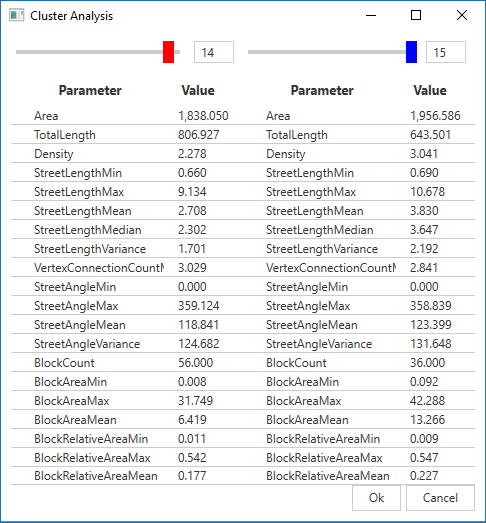
\includegraphics[width=0.8\linewidth]{cluster_applied_compare.png}
    \caption{This gui dialog allows to select two clusters and to compare the measured values.}
    \label{fig:applied_clustering_analysis_GUI}
\end{figure}

\begin{figure}[ht]
    \centering
    \begin{mdframed}[style=border]
        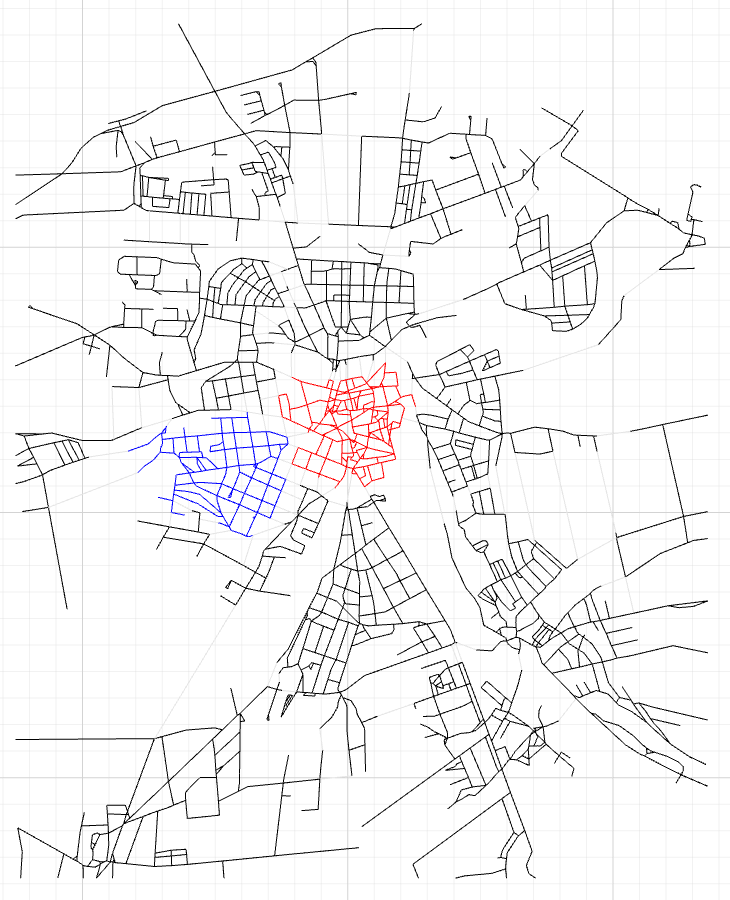
\includegraphics[width=\linewidth]{cluster_applied_compare_visualized.png}
    \end{mdframed}
    \caption{Main view with marked from the 'Cluster Analysis' dialog}
    \label{fig:applied_clustering_analysis_visualized_GUI}
\end{figure}

\FloatBarrier
\section{Measured Clusters}
\label{sec:measurements_full_table}
This table represent the full measured data with the cluster analysis method.

\begin{table}[h]
    \begin{center}
        \begin{tabular}{ |l|l|l|l|l| }
            \hline
            \textbf{Parmate}r &
            & \textbf{C1} \ref{sec:historyDistinct}
            & \textbf{C2} \ref{sec:businessDistinct}
            & \textbf{C3} \ref{sec:outskits}  \\ 
            \hline
            \multirow{4}{*}{Total} 
            & Area & 1838.05 & 1956.59 & 7802.74 \\
            & Length & 806.92 & 643.50 & 1069.81 \\
            & Density & 2.28 & 3.04 & 7.29 \\
            \hline
            \multirow{5}{*}{Street Length}
            & Min & 0.66 & 0.69 & 0.73 \\
            & Max & 9.13 & 10.68 & 38.00 \\
            & Mean & 2.72 & 3.85 & 4.82 \\
            & Median & 2.30 & 3.65 & 3.28 \\
            & Variance & 1.70 & 2.19 & 5.00 \\
            \hline
            \multirow{1}{*}{Vertex} 
            & Connections & 3.04 & 2.84 & 2.45 \\
            \hline
            \multirow{5}{*}{Street Angle} 
            & Min & 0.00 & 0.00 & 0.00 \\
            & Max & 151.80 & 358.84 & 359.80 \\
            & Mean & 119.03 & 123.75 & 137.18 \\
            & Variance & 124.68 & 131.65 & 129.47 \\
            \hline
            \multirow{5}{*}{Block} 
            & Count & 55 & 35 & 26 \\
            & Area Min & 0.01 & 0.09 & 0.00 \\
            & Area Max & 31.75 & 42.29 & 567.26 \\
            & Area Mean & 6.54 & 13.65 & 76.30 \\
            & A/Ac Min & 0.01 & 0.01 & 0.00 \\
            & A/Ac Max & 0.54 & 0.55 & 0.66 \\
            & A/Ac Mean & 0.18 & 0.23 & 0.18 \\
            \hline
            \multirow{5}{*}{Integration} 
            & Min & 0.46 & 0.48 & 0.60 \\
            & Max & 0.57 & 0.75 & 1.0 \\
            & Mean & 0.49 & 0.59 & 0.78 \\
            \hline
            \multirow{5}{*}{Choice}
            & Min & 0.00 & 0.00 & 0.00 \\
            & Max & 1.00 & 0.67 & 0.34 \\
            & Mean & 0.10 & 0.05 & 0.04 \\
            \hline
        \end{tabular}
        \caption{Measured results from Historic District (C1) \ref{sec:historyDistinct}, Business District (C2) \ref{sec:businessDistinct} and Outskirts Area (C3) \ref{sec:outskits}}
    \end{center}
\end{table}

\end{document}